%%%%%%%%%%%%%%%%%%%%%%%%%%%%%%%%%%%%%%%%%%%%%%%%%%%%%%%%%%%%%%%
%% OXFORD THESIS TEMPLATE

% Use this template to produce a standard thesis that meets the Oxford University requirements for DPhil submission
%
% Originally by Keith A. Gillow (gillow@maths.ox.ac.uk), 1997
% Modified by Sam Evans (sam@samuelevansresearch.org), 2007
% Modified by John McManigle (john@oxfordechoes.com), 2015
% Modified by Ulrik Lyngs (ulrik.lyngs@cs.ox.ac.uk), 2018-, for use with R Markdown
%
% Ulrik Lyngs, 25 Nov 2018: Following John McManigle, broad permissions are granted to use, modify, and distribute this software
% as specified in the MIT License included in this distribution's LICENSE file.
%
% John commented this file extensively, so read through to see how to use the various options.  Remember that in LaTeX,
% any line starting with a % is NOT executed.

%%%%% PAGE LAYOUT
% The most common choices should be below.  You can also do other things, like replace "a4paper" with "letterpaper", etc.

% 'twoside' formats for two-sided binding (ie left and right pages have mirror margins; blank pages inserted where needed):
%\documentclass[a4paper,twoside]{templates/ociamthesis}
% Specifying nothing formats for one-sided binding (ie left margin > right margin; no extra blank pages):
%\documentclass[a4paper]{ociamthesis}
% 'nobind' formats for PDF output (ie equal margins, no extra blank pages):
%\documentclass[a4paper,nobind]{templates/ociamthesis}

% As you can see from the line below, oxforddown uses the a4paper size, 
% and passes in the binding option from the YAML header in index.Rmd:
\documentclass[a4paper, nobind]{templates/ociamthesis}


%%%%% ADDING LATEX PACKAGES
%FONTS
\usepackage{times}
% add hyperref package with options from YAML %
\usepackage[pdfpagelabels]{hyperref}
% handle long urls
\usepackage{xurl}
% change the default coloring of links to something sensible
\usepackage{xcolor}



\definecolor{mylinkcolor}{RGB}{0,0,139}
\definecolor{myurlcolor}{RGB}{0,0,139}
\definecolor{mycitecolor}{RGB}{0,33,71}

\hypersetup{
  hidelinks,
  colorlinks,
  linktocpage=true,
  linkcolor=mylinkcolor,
  urlcolor=myurlcolor,
  citecolor=mycitecolor
}


% add float package to allow manual control of figure positioning %
\usepackage{float}

% enable strikethrough
\usepackage[normalem]{ulem}

% use soul package for correction highlighting
\usepackage{color, soulutf8}
\definecolor{correctioncolor}{HTML}{CCCCFF}
\sethlcolor{correctioncolor}
\newcommand{\ctext}[3][RGB]{%
  \begingroup
  \definecolor{hlcolor}{#1}{#2}\sethlcolor{hlcolor}%
  \hl{#3}%
  \endgroup
}
% stop soul from freaking out when it sees citation commands
\soulregister\ref7
\soulregister\cite7
\soulregister\citet7
\soulregister\autocite7
\soulregister\textcite7
\soulregister\pageref7

%%%%% FIXING / ADDING THINGS THAT'S SPECIAL TO R MARKDOWN'S USE OF LATEX TEMPLATES
% pandoc puts lists in 'tightlist' command when no space between bullet points in Rmd file,
% so we add this command to the template
\providecommand{\tightlist}{%
  \setlength{\itemsep}{0pt}\setlength{\parskip}{0pt}}
 
% allow us to include code blocks in shaded environments

% User-included things with header_includes or in_header will appear here
% kableExtra packages will appear here if you use library(kableExtra)
\usepackage{booktabs}
\usepackage{longtable}
\usepackage{array}
\usepackage{multirow}
\usepackage{wrapfig}
\usepackage{float}
\usepackage{colortbl}
\usepackage{pdflscape}
\usepackage{tabu}
\usepackage{threeparttable}
\usepackage{threeparttablex}
\usepackage[normalem]{ulem}
\usepackage{makecell}
\usepackage{xcolor}


%UL set section header spacing
\usepackage{titlesec}
% 
\titlespacing\subsubsection{0pt}{24pt plus 4pt minus 2pt}{0pt plus 2pt minus 2pt}


%UL set whitespace around verbatim environments
\usepackage{etoolbox}
\makeatletter
\preto{\@verbatim}{\topsep=0pt \partopsep=0pt }
\makeatother


%%%%%%% PAGE HEADERS AND FOOTERS %%%%%%%%%
\usepackage{fancyhdr}
\setlength{\headheight}{15pt}
\fancyhf{} % clear the header and footers
\pagestyle{fancy}
\renewcommand{\chaptermark}[1]{\markboth{\thechapter. #1}{\thechapter. #1}}
\renewcommand{\sectionmark}[1]{\markright{\thesection. #1}} 
\renewcommand{\headrulewidth}{0pt}

\fancyhead[LO]{\emph{\leftmark}} 
\fancyhead[RE]{\emph{\rightmark}} 




% UL page number position 
\fancyfoot[C]{\emph{\thepage}} %regular pages
\fancypagestyle{plain}{\fancyhf{}\fancyfoot[C]{\emph{\thepage}}} %chapter pages




%%%%% SELECT YOUR DRAFT OPTIONS
% This adds a "DRAFT" footer to every normal page.  (The first page of each chapter is not a "normal" page.)

% IP feb 2021: option to include line numbers in PDF

% for line wrapping in code blocks
\usepackage{fancyvrb}
\usepackage{fvextra}
\DefineVerbatimEnvironment{Highlighting}{Verbatim}{breaklines=true, breakanywhere=true, commandchars=\\\{\}}

% for quotations -- loaded here rather than in ociamthesis.cls, as it needs to
% be loaded after fvextra, otherwise we get a warning message
\usepackage{csquotes}

% This highlights (in blue) corrections marked with (for words) \mccorrect{blah} or (for whole
% paragraphs) \begin{mccorrection} . . . \end{mccorrection}.  This can be useful for sending a PDF of
% your corrected thesis to your examiners for review.  Turn it off, and the blue disappears.
\correctionstrue


%%%%% BIBLIOGRAPHY SETUP
% Note that your bibliography will require some tweaking depending on your department, preferred format, etc.
% If you've not used LaTeX before, I recommend just using pandoc for citations -- this is what's used unless you specific e.g. "citation_package: natbib" in index.Rmd
% If you're already a LaTeX pro and are used to natbib or something, modify as necessary.

% this allows the latex template to handle pandoc citations
\newlength{\cslhangindent}
\setlength{\cslhangindent}{1.5em}
\newlength{\csllabelwidth}
\setlength{\csllabelwidth}{3em}
\newlength{\cslentryspacingunit} % times entry-spacing
\setlength{\cslentryspacingunit}{\parskip}
\newenvironment{CSLReferences}[2] % #1 hanging-ident, #2 entry spacing
 {% don't indent paragraphs
  \setlength{\parindent}{0pt}
  % turn on hanging indent if param 1 is 1
  \ifodd #1
  \let\oldpar\par
  \def\par{\hangindent=\cslhangindent\oldpar}
  \fi
  % set entry spacing
  \setlength{\parskip}{1mm}
  \setlength{\baselineskip}{6mm}
 }%
 {}
\usepackage{calc}
\newcommand{\CSLBlock}[1]{#1\hfill\break}
\newcommand{\CSLLeftMargin}[1]{\parbox[t]{\csllabelwidth}{#1}}
\newcommand{\CSLRightInline}[1]{\parbox[t]{\linewidth - \csllabelwidth}{#1}\break}
\newcommand{\CSLIndent}[1]{\hspace{\cslhangindent}#1}




% Uncomment this if you want equation numbers per section (2.3.12), instead of per chapter (2.18):
%\numberwithin{equation}{subsection}


%%%%% THESIS / TITLE PAGE INFORMATION
% Everybody needs to complete the following:
\title{\textquestiondown Vamos bien?\\
\emph{Valoración de las Políticas Públicas Europeas del sector agrario por parte de agricultores de tomate ecológico en Andalucía y Extremadura}}
\author{Ignacio Pastore Benaim}
% 

% Master's candidates who require the alternate title page (with candidate number and word count)
% must also un-comment and complete the following three lines:

% Uncomment the following line if your degree also includes exams (eg most masters):
%\renewcommand{\submittedtext}{Submitted in partial completion of the}
% Your full degree name.  (But remember that DPhils aren't "in" anything.  They're just DPhils.)
\degree{Máster en Agricultura y Ganadería Ecológica}

% Term and year of submission, or date if your board requires (eg most masters)
\degreedate{Octubre 2023}


%%%%% YOUR OWN PERSONAL MACROS
% This is a good place to dump your own LaTeX macros as they come up.

% To make text superscripts shortcuts
\renewcommand{\th}{\textsuperscript{th}} % ex: I won 4\th place
\newcommand{\nd}{\textsuperscript{nd}}
\renewcommand{\st}{\textsuperscript{st}}
\newcommand{\rd}{\textsuperscript{rd}}

%%%%% THE ACTUAL DOCUMENT STARTS HERE
\begin{document}

%%%%% CHOOSE YOUR LINE SPACING HERE
% This is the official option.  Use it for your submission copy and library copy:
% \setlength{\textbaselineskip}{22pt plus2pt}
% This is closer spacing (about 1.5-spaced) that you might prefer for your personal copies:
\setlength{\textbaselineskip}{18pt plus2pt minus1pt}

% You can set the spacing here for the roman-numbered pages (acknowledgements, table of contents, etc.)
\setlength{\frontmatterbaselineskip}{17pt plus1pt minus1pt}

% UL: You can set the line and paragraph spacing here for the separate abstract page to be handed in to Examination schools
\setlength{\abstractseparatelineskip}{13pt plus1pt minus1pt}
\setlength{\abstractseparateparskip}{0pt plus 1pt}

% UL: You can set the general paragraph spacing here - I've set it to 2pt (was 0) so
% it's less claustrophobic
\setlength{\parskip}{2pt plus 1pt}

%
% Customise title page
%
\def\crest{{\includegraphics[width=5cm]{templates/logo\_unia.png}}}
\renewcommand{\university}{Universidad Internacional de Andalucía}
\renewcommand{\submittedtext}{}
\renewcommand{\thesistitlesize}{\fontsize{22pt}{28pt}\selectfont}
\renewcommand{\gapbeforecrest}{25mm}
\renewcommand{\gapaftercrest}{25mm
}


% Leave this line alone; it gets things started for the real document.
\setlength{\baselineskip}{\textbaselineskip}


%%%%% CHOOSE YOUR SECTION NUMBERING DEPTH HERE
% You have two choices.  First, how far down are sections numbered?  (Below that, they're named but
% don't get numbers.)  Second, what level of section appears in the table of contents?  These don't have
% to match: you can have numbered sections that don't show up in the ToC, or unnumbered sections that
% do.  Throughout, 0 = chapter; 1 = section; 2 = subsection; 3 = subsubsection, 4 = paragraph...

% The level that gets a number:
\setcounter{secnumdepth}{2}
% The level that shows up in the ToC:
\setcounter{tocdepth}{1}


%%%%% ABSTRACT SEPARATE
% This is used to create the separate, one-page abstract that you are required to hand into the Exam
% Schools.  You can comment it out to generate a PDF for printing or whatnot.

% JEM: Pages are roman numbered from here, though page numbers are invisible until ToC.  This is in
% keeping with most typesetting conventions.
\begin{romanpages}

% Title page is created here
\maketitle

%%%%% DEDICATION

%%%%% ACKNOWLEDGEMENTS


\begin{acknowledgements}
 	\centering

 \vspace{30mm}

 Agradezco a mis tutores Gloria y Pau por guiarme con el escrito del presente trabajo durante mi estadía en Sevilla.

 \vspace{10mm}

 Gracias a la compañera Laura por ayudarme con el análisis estadístico.

 \vspace{10mm}

 Profundo agradecimiento a los agricutlores y agricultoras que con humildad me recibieron con los brazos abiertos y llenaron mi alacena con alimento sano y soberano.

 \vspace{10mm}

 Gracias a todos y a todas las que hacen posible que pueda dedicarme a aportar mi granito de arena.

 \vspace{10mm}

 A la Madre Tierra por nutrirnos y sostenernos.

 \vfill

 \begin{flushright}
 Ignacio Pastore Benaim \\
 11 Octubre 2023
 \end{flushright}
\end{acknowledgements}



%%%%% ABSTRACT


\renewcommand{\abstracttitle}{Resumen}
\begin{abstract}
	\setlength{\baselineskip}{30pt}

Es indudable de que estamos atravesando una crisis ecosocial globalizada. La agroecología política propone la transformación del regimen agroalimentario dominante como medida más efectiva para atravesar la crisis. En el marco de un proyecto financiado por el Centro Común de Investigación Europea se realizaron 55 entrevistas en campo con el fin de conocer la percepción de los agricultores acerca de las Políticas Públicas Europeas del sector agrario. Según un análisis estadístico se realizó el diagnóstico del actual marco normativo y se sacaron conclusiones para mejorar el alcance de las Políticas Públicas en vistas catalizar la transición hacia un nuevo régimen agroalimentario de base agroecológica.
\end{abstract}


\phantomsection

\renewcommand{\abstractsecondtitle}{Abstract}
\begin{abstractsecond}
	\setlength{\baselineskip}{30pt}

It is undeniable that we are going through a globalized ecosocial crisis. Political agroecology proposes the transformation of the dominant agri-food regime as the most effective measure to navigate the crisis. Within the framework of a project funded by the European Joint Research Centre, 55 field interviews were conducted to understand farmers' perceptions of European Public Policies in the agricultural sector. Through statistical analysis, a diagnosis of the current regulatory framework was carried out, and conclusions were drawn to enhance the scope of Public Policies with a view to catalyzing the transition towards a new agroecologically based agri-food regime
\end{abstractsecond}


%TRADUCCION
% \listoffigures:
\renewcommand\listfigurename{Lista de Figuras}   % capitalization required by Guide
% \listoftables:
\renewcommand\listtablename{Lista de Tablas}


%%%%% MINI TABLES
% This lays the groundwork for per-chapter, mini tables of contents.  Comment the following line
% (and remove \minitoc from the chapter files) if you don't want this.  Un-comment either of the
% next two lines if you want a per-chapter list of figures or tables.
\dominitoc % include a mini table of contents

% This aligns the bottom of the text of each page.  It generally makes things look better.
\flushbottom

%TRADUCCION
\renewcommand{\contentsname}{Índice}

% This is where the whole-document ToC appears:
\tableofcontents

\listoffigures
	\mtcaddchapter
  	% \mtcaddchapter is needed when adding a non-chapter (but chapter-like) entity to avoid confusing minitoc

% Uncomment to generate a list of tables:
\listoftables
  \mtcaddchapter
%%%%% LIST OF ABBREVIATIONS
% This example includes a list of abbreviations.  Look at text/abbreviations.tex to see how that file is
% formatted.  The template can handle any kind of list though, so this might be a good place for a
% glossary, etc.
% First parameter can be changed eg to "Glossary" or something.
% Second parameter is the max length of bold terms.
\begin{mclistof}{Lista de Abreviaciones}{3.2cm}

\item[CCI]

Centro Común de Investigación.

\item[UE]

Unión Europea.

\item[MIP]

Manejo Integral de Plagas.

\item[PVE]

Pacto Verde Europeo.

\item[ONU]

Organización de las Naciones Unidas.

\item[PPs]

Políticas Públicas.

\item[FAO]

Organización de las Naciones Unidas para la Agricultura y la Alimentación.

\item[ODS]

Objetivos de Desarrollo Sustentable.

\item[SAU]

Superficie Agrícola Utilizada.

\end{mclistof} 


% The Roman pages, like the Roman Empire, must come to its inevitable close.
\end{romanpages}

%%%%% CHAPTERS
% Add or remove any chapters you'd like here, by file name (excluding '.tex'):
\flushbottom

%TRADUCCION
\renewcommand\tablename{Tabla}
\renewcommand\figurename{Figura}
% \renewcommand{\appendixname}{Anexo}
\renewcommand{\appendixtocname}{Anexos}
\renewcommand{\appendixpagename}{Anexos}

% all your chapters and appendices will appear here
\sloppy
\hypertarget{introduccion}{%
\chapter{Introducción}\label{introduccion}}

\minitoc

\hypertarget{como_llegamos}{%
\section{\texorpdfstring{\textquestiondown Cómo llegamos hasta acá?}{Cómo llegamos hasta acá?}}\label{como_llegamos}}

La alimentación es uno de los nexos principales entre un individuo y su
entorno. El ser humano interviene en los ciclos naturales de nutrientes
y energía para asegurar su supervivencia. Desde los humanos más
primitivos, hace unos 2.5 millones de años, esta relación estaba
dominada por un sistema de caza y recolección. Con el advenimiento de la
agricultura, hace 12.000 años, las intervenciones del ser humano en los
sistemas ecológicos se intensificaron. De un sistema nómada de caza y
recolección se pasó a un sistema sedentario motorizado por la energía
solar, captada por la fotosíntesis, el trabajo animal y la mano de obra
humana. Así, la agricultura permitió la aparición de las primeras
civilizaciones sedentarias donde tuvieron lugar los primeros
intercambios comerciales. Con esto, la alimentación además de ser un
nexo con el entorno natural se convirtió en una vinculación entre
individuos.

A finales del siglo XVIII con la llegada de la revolución industrial el
ser humano potenció su capacidad de transformación del entorno,
iniciando una época geológica denominada ``Antropoceno'', cuya principal
fuente de cambio geológico es la actividad humana (Crutzen \& Stoermer, 2021).

Durante el siglo XX, la industrialización de la agricultura reconfiguró
radicalmente las fuerzas motoras de los sistemas agrícolas. La energía
solar fue suplantada por energía de base fósil y el trabajo animal y
mano de obra humana fue suplantada por maquinaria agrícola
(Agnoletti, 2006; González de Molina \& Toledo, 2014; Guzmán Casado \& González De Molina, 2009).

En la década de 1960, el aporte biotecnológico a la agricultura dio
lugar a la \emph{Revolución Verde}. A partir de la introducción de un paquete
tecnológico formado por variedades de semillas mejoradas, pesticidas y
fertilizantes inorgánicos, la producción agropecuaria se
super-intensificó permitiendo aumentar la producción global de alimentos
muy por encima del crecimiento de la población mundial
(IPCC, 2019). La agricultura resultante de estas prácticas es
llamada \emph{Agricultura Convencional} y es la que rige el sistema
agroalimentario actual (Guzmán Casado et al., 2000).

Hoy la actual crisis civilizadora global, marca la necesidad de
reformular el desarrollo socioeconómico, donde el sistema
agroalimentario es la pieza clave por constituir la mayor fuerza motriz
de las transformaciones biofísicas del Planeta Tierra (Foley et al., 2005; Tilman et al., 2001; Weis, 2013).

\hypertarget{colapso}{%
\section{\texorpdfstring{Crónica de un Colapso anunciado: \textquestiondown De qué hablamos cuando hablamos de crisis?}{Crónica de un Colapso anunciado: De qué hablamos cuando hablamos de crisis?}}\label{colapso}}

Cada vez es más evidente que estamos atravesando una crisis estructural
(Garrido Peña et al., 2007; Toledo, 2012) que expone los límites
de nuestra civilización. A continuación se desarrollan algunos de ellos.

\hypertarget{biofisicos}{%
\subsection{Límites biofísicos}\label{biofisicos}}

La comunidad científica ha identificado límites planetarios que de
sobrepasarse complican la regeneración de los sistemas ecológicos que
sustentan las condiciones necesarias para el desarrollo de la vida
humana (Rockstrom et al., 2009).

Cinco de los nueve límites desarrollados por Rockström ya fueron
sobrepasados: la interferencia en el ciclo del nitrógeno y el fósforo;
el uso y contaminación del agua; el uso y degradación de los suelos; el
cambio climático y la pérdida de biodiversidad (Steffen et al., 2015). Con
excepción del cambio climático, la agricultura es la principal
influencia de estos cinco límites (Campbell et al., 2017).

\hypertarget{limities_econuxf3micos}{%
\subsection{Límites físicos al crecimiento económico}\label{limities_econuxf3micos}}

En el 2022, según el Banco Mundial, el mercado de commodities sufrió una
gran suba de precios, llevando a algunas materias primas a sus precios
máximos históricos (World Bank, 2022). Por un lado, este shock
inflacionario puede ser atribuido a una nueva guerra, la de Ucrania y
Rusia, donde Ucrania es exportador neto de granos y fertilizantes
químicos. En este contexto, el régimen agroalimentario vuelve a mostrar
su talón de Aquiles, la globalización y su falta de resiliencia debido a
la integración vertical de sus procesos.

Sin embargo, no se debe perder de vista el agotamiento de los recursos
naturales como variable determinante en la inflación de los precios de
las materias primas. Según la teoría de Hubbert (Hubbert M, 1956), la
extracción de recursos no-renovables tiene un pico, que luego de haberlo
pasado, la tasa de beneficio de extracción por unidad de material
decrece. En otras palabras, a mayor escasez, más costoso es la
extracción del material y, por ende, más caro su utilización. Por
ejemplo, cada vez es más costoso extraer una tonelada de petróleo
(Hall et al., 2009; Hall, 2011; Laherrère et al., 2022). Pero
lamentablemente este no es el único caso, una situación similar sucede
con el fósforo (Cordell, 2010), hierro, aluminio y cobre
(Valero Capilla \& Valero Delgado, 2015) y otros recursos renovables como la madera
(Shearman et al., 2012) y el agua (Aguilera et al., 2019).

El crecimiento económico durante el siglo XX sostenido por las materias
primas baratas se topó con la finitud de los recursos
(I. UNEP, 2011; I. UNEP et al., 2016) y, en consecuencia, la alta
dependencia de insumos externos al régimen agroalimentario limita
rotundamente la sostenibilidad del mismo.

\hypertarget{hambre}{%
\subsection{El hambre como límite: inseguridad alimentaria}\label{hambre}}

Según la FAO, en el 2022, 2.400 millones de personas sufrieron de
inseguridad alimentaria alta o moderada (29,6\% de la población mundial y
más de 391 millones de personas que en 2019). Además, se estima que
entre 690 y 783 millones de personas sufrieron de hambre (alrededor del
9\% de la población mundial y más de 3,8 millones que en 2021)
(FAO, 2023).

Pese a que actualmente se producen alimentos suficientes para alimentar
a toda la población mundial, el régimen agroalimentario no consigue
cumplir con lo que debería ser su objetivo principal. Parece ser que su
fin es otro, convertir el alimento en mercancía.

\hypertarget{abandono_tierras}{%
\subsection{Abandono de tierras y recambio generacional}\label{abandono_tierras}}

El fenómeno de intensificación y concentración también afecta al diseño
demográfico del paño campo-ciudad. En 1950 el 30 \% de la población vivía
en ciudades, para el 2021 este número aumentó a 57\% y se proyecta que
para 2050 siete de cada diez personas vivan en la ciudad (FAO, 2023).

Estos números dejan entrever dos síntomas que imperan atenderse: el
abandono de tierras y la falta de recambio generacional en las familias
productoras. La expansión del monocultivo y la globalización alimentaria
ha llevado a la ruina a millones de productores, provocando el abandono
de tierras (González de Molina et al., 2021). Además, las presiones económicas hacia los
pequeños productores limita el horizonte de bienestar de los jóvenes que
deciden emigrar hacia las ciudades en búsqueda de prosperidad económica.

Es importante remarcar que la población urbana se alimenta de lo que se
produce en zonas rurales. De profundizarse este pronóstico se pone en
riesgo el acceso a alimentos, agravando el estado de la seguridad
alimentaria y perdiendo definitivamente la soberanía alimentaria de los
pueblos.

\hypertarget{quiendijoperdido}{%
\section{\texorpdfstring{\textquestiondown Quién dijo que todo está perdido? Agroecología como solución}{Quién dijo que todo está perdido? Agroecología como solución}}\label{quiendijoperdido}}

Ante semejante panorama desesperanzador la Agroecología se presenta como
un marco teórico-práctico que busca dar soluciones de manera holística a
los grandes desafíos a los que nos enfrentamos hoy.

\hypertarget{historia_agroecologia}{%
\subsection{Un poco de historia}\label{historia_agroecologia}}

La primera vez que se utilizó el término agroecología en el ambiente
académico fue en el año 1928 por Bensin (Bensin, 1928). En
un principio y, como lo indica la composición del término, se trataba de
la fusión de dos áreas de conocimiento hasta el momento separadas: la
agricultura y la ecología. Hasta finales de los 60s la utilización del
término se refirió a la parte práctica, un conjunto de técnicas para
producir de manera sostenible a nivel parcela. La agroecología entendida
como la ecología aplicada a la producción de plantas y la gestión de
tierras agrícolas (Hénin, 1967).

A partir de los 70s, la noción de la agroecología se expandió
probablemente como respuesta a la \emph{Revolución Verde}
(Hecht, 1995; Shiva, 1989). Por un lado, se
intensificaron los estudios de las prácticas derivadas de la aplicación
de la ecología a los agroecosistemas (Altieri, 1987; Gliessman, 1990) y, en paralelo, emergieron escuelas de
pensamiento y movimientos que reivindicaban las prácticas agroecológicas
como principal vector de desarrollo rural .

Hacia 1990, se volvió a ampliar el alcance, pasando de la escala de los
agroecosistemas a nivel local a los sistemas agroalimentarios
(Wezel \& Soldat, 2009), entendidos como redes de producción, procesamiento,
distribución y consumo de alimentos que se estructuran desde el nivel
local hasta la escala global.

Para superar los desafíos de crecimiento de escala, la agroecología ha
ido combinando sinérgicamente estas tres dimensiones de acción: como
ciencia, práctica y movimiento social. Por tanto, la agroecología debe
entenderse como una ``\emph{ciencia transformadora}'' (Levidow et al., 2014; Schneidewind et al., 2016), o ``\emph{ciencia digna}'' (Carrasco, Andrés E., 2014),
es decir, un enfoque transdisciplinario basado en principios de la
sostenibilidad socioeconómica (Méndez et al., 2013) que busca transformar el
régimen agroalimentario (Holt-Giménez \& Altieri, 2013; McMichael, 2006).

\hypertarget{agroecologia_politica}{%
\subsection{A seguir escalando: Agroecología Política}\label{agroecologia_politica}}

Las raíces de la crisis del régimen agroalimentario no son los impactos
socioambientales sino el marco institucional que lo gobierna. No hay que
confundir las causas con las consecuencias, es menester un cambio
profundo en el marco institucional vigente para que las experiencias
agroecológicas prosperen y se mantengan en el tiempo (González de Molina et al., 2021).

El punto de inflexión de la inclusión de la agroecología en el diseño de
políticas públicas probablemente surgió con la publicación del IAASTD
reconociendo a la agroecología como una ``alternativa'' prometedora para
resolver los problemas del hambre, pobreza rural y desarrollo sostenible
(International Assessment of Agricultural Knowledge Science and Technology for Development (IAASTD), 2009). Luego, otros organismos de las Naciones Unidas publicaron
documentos reforzando el potencial transformador de la agroecología
(De Schutter et al., 2011; HLPE, 2017).

Por ende, la agroecología política tiene como objetivo el diseño de
instituciones (Ostrom, 1990, 2009; Ostrom, 2001)
que favorezcan la sustentabilidad agraria. Se trata, pues, de
metamorfosear el marco institucional impuesto por el régimen alimentario
mediante el salto de escala de las experiencias agroecológicas. Las
políticas públicas constituyen un instrumento imprescindible para
generar un nuevo marco normativo próspero que sustente y multiplique las
experiencias agroecológicas locales hasta generar una masa crítica capaz
de generar un nuevo régimen agroalimentario sustentable.

\hypertarget{agricultura-familiar}{%
\subsection{Actores principales: campesinado y familias productoras}\label{agricultura-familiar}}

La forma mayoritaria de organizar la producción mundial de alimentos es
la agricultura familiar. Alrededor del 75\% de las tierras agrícolas son
manejadas por agricultores familiares (Lowder et al., 2016). Eso significa que
la agricultura familiar es la fuerza sociomaterial y cultural sobre la
cual debe basarse la propuesta agroecológica.

Resulta obvio pensar en que cualquier estrategia que haga avanzar la
transición, masificando las experiencias agroecológicas y construyendo
un régimen alimentario alternativo debe basarse en los campesinos.

\hypertarget{prouesta_trabajo}{%
\section{Propuesta de Trabajo}\label{prouesta_trabajo}}

Este Trabajo Final de Máster propone estudiar la opinión de los
agricultores ecológicos locales de Andalucía y Extremadura acerca de
algunas políticas públicas (PPs) de la UE relacionadas con el regimen
agroalimentario. Para acotar el alcance del trabajo, se limitó la
elección de los entrevistados a agricultores de un cultivo
característico de la zona, el tomate.\\
Se evaluará el rumbo de la transición agroecológica a través de la
alineación del marco normativo a un nuevo régimen agroalimentario.
Finalmente se sacarán conclusiones para el diseño de futuras PPs que
puedan catalizar la transformación.

\hypertarget{PPs}{%
\subsection{Políticas Públicas de la UE a analizar}\label{PPs}}

En el contexto descripto en la sección \ref{colapso}, la Unión Europea
ha trazado estrategias trasnacionales para afrontar los desafíos
ambientales celebrando a fines del 2019 el \emph{``Pacto Verde Europeo'' (PVE)}
\footnote{\href{https://eur-lex.europa.eu/legal-content/ES/TXT/?uri=COM\%3A2019\%3A640\%3AFIN}{Comunicación de la Comisión Al Parlamento
  Europeo, al Consejo Europeo, al Consejo, al Comité Económico y
  Social Europeo y al Comité de Las Regiones: El Pacto Verde Europeo
  {[}(COM(2019)640
  final{]}}}. Según explica el documento de divulgación del
\emph{PVE}:

\begin{quote}
\emph{``Se trata de una nueva estrategia de crecimiento destinada a
transformar la UE en una sociedad equitativa y próspera, con una
economía moderna, eficiente en el uso de los recursos y competitiva,
en la que no habrá emisiones netas de gases de efecto invernadero en
2050 y el crecimiento económico estará disociado del uso de los
recursos.''}
\end{quote}

Las estrategias dentro del \emph{PVE} con mayor relación al sector
agroalimentario y al presente trabajo son las siguientes:

\begin{itemize}
\tightlist
\item
  Estrategia de la granja a la mesa.
\item
  Directiva del uso sostenible de plaguicidas.
\item
  Estrategia sobre la biodiversidad.
\end{itemize}

Además de las 3 normas anteriores se analizarán otras PPs relevantes
para el sector agroalimentario español:

\begin{itemize}
\tightlist
\item
  Directiva de Nitratos.
\item
  Directiva de Hábitats y Directiva de Aves.
\item
  Directiva del Marco del Agua.
\end{itemize}

A continuación se realiza una breve descripción de cada una de ellas.

\hypertarget{granja-mesa}{%
\subsubsection{Estrategia de la Granja a la Mesa}\label{granja-mesa}}

En la primavera de 2020 se lanza la estrategia ``De la granja a la mesa''
\footnote{\href{https://eur-lex.europa.eu/legal-content/ES/TXT/?qid=1693563760418&uri=CELEX\%3A52020DC0381}{Comunicación de la Comisión Al Parlamento
  Europeo, al Consejo Europeo, al Consejo, al Comité Económico y
  Social Europeo y al Comité de Las Regiones: Estrategia ``de la granja
  a la mesa'' para un sistema alimentario justo, saludable y respetuoso
  con el medio ambiente {[}(COM(2020)381
  final{]}}} donde se tratan ampliamente los desafíos para
alcanzar un sistema alimentario sostenible.\\

En general se reconoce que para alcanzar los desafíos ambientales del
\emph{PVE} y los \emph{Objetivos de Desarrollo Sustentable (ODS)} de la \emph{ONU} es
necesario actuar a gran escala, integrando las diferentes partes del
régimen agroalimentario:

\begin{quote}
\emph{``\ldots{} garantizar que la cadena alimentaria, que abarca la producción,
el transporte, la distribución, la comercialización y el consumo de
alimentos, tenga un impacto medioambiental neutro o positivo, y
preservar y restablecer los recursos terrestres, de agua dulce y
marinos de los que depende el sistema alimentario.''}
\end{quote}

En particular, especifica medidas en torno a la producción: técnicas de
cultivo, ingreso de los agricultores y uso de plaguicidas.

\begin{quote}
\emph{``La Comisión tomará medidas adicionales para reducir el uso y el
riesgo globales de los plaguicidas químicos en un 50 \%, así como el
uso de los plaguicidas más peligrosos en un 50 \% de aquí a 2030 \ldots{}
Revisará la Directiva sobre el uso sostenible de los plaguicidas,
mejorará las disposiciones relativas a la gestión integrada de plagas
(GIP) y promoverá un mayor uso de métodos alternativos seguros para
proteger las cosechas de plagas y enfermedades.''}
\end{quote}

\hypertarget{directiva-sobre-el-uso-sostenible-de-plaguicidas}{%
\subsubsection{Directiva sobre el uso sostenible de plaguicidas}\label{directiva-sobre-el-uso-sostenible-de-plaguicidas}}

En el año 2009 se instrumentó la Directiva 2009/128/CE
\footnote{\href{https://eur-lex.europa.eu/legal-content/ES/TXT/?uri=celex\%3A32009L0128}{Directiva 2009/128/CE del Parlamento Europeo y
  del Consejo, de 21 de octubre de 2009 , por la que se establece el
  marco de la actuación comunitaria para conseguir un uso sostenible
  de los plaguicidas (Texto pertinente a efectos del
  EEE)}}estableciendo un marco para conseguir un uso
sostenible de los plaguicidas mediante la reducción de los riesgos y los
efectos de la utilización de plaguicidas en la salud humana y en el
medio ambiente.

Sin embargo la evaluación de su aplicación no fue satisfactoria según
los informes de la Comisión al Parlamento Europeo y al Consejo de
2017\footnote{Informe de la Comisión al Parlamento Europeo y al
  Consejo sobre los planes de acción nacionales de los Estados
  miembros y sobre los avances en la aplicación de la Directiva
  2009/128/CE, relativa al uso sostenible de los plaguicidas
  {[}COM(2017) 587 final{]}.} y 2020\footnote{\href{https://eur-lex.europa.eu/legal-content/ES/TXT/?uri=CELEX\%3A52020DC0204&qid=1693565338135}{Informe de la Comisión al Parlamento Europeo y al
  Consejo sobre la experiencia adquirida por los Estados miembros con
  la aplicación de los objetivos nacionales establecidos en sus planes
  de acción nacionales y sobre los avances conseguidos en la
  aplicación de la Directiva 2009/128/CE relativa al uso sostenible de
  los plaguicidas {[}COM(2020) 204
  final{]}}}. A través de la
estrategia ``De la Granja a la Mesa'' se estableció en el año 2022 la
última actualización de esta directiva delineando nuevos objetivos:\\

\begin{quote}
\emph{``Objetivos de reducción de la Unión para 2030 de productos
fitosanitarios químicos:\\
\strut \\
1 - Cada Estado miembro contribuirá, mediante la adopción y la
consecución de sus objetivos nacionales de conformidad con el artículo
5, a lograr, de aquí a 2030, una reducción del 50 \% a escala de la
Unión tanto del uso como del riesgo de los productos fitosanitarios
químicos (objetivo 1 de reducción de la Unión para 2030) y del uso de
los productos fitosanitarios más peligrosos (objetivo 2 de reducción
de la Unión para 2030), en comparación con la media de los años 2015,
2016 y 2017 (denominados conjuntamente los objetivos de reducción de
la Unión para 2030).\\
\strut \\
2 - La Comisión calculará anualmente los avances hacia la consecución
de los objetivos de reducción de la Unión para 2030 de conformidad con
la metodología establecida en el anexo I.''}
\end{quote}

\hfill\break
Como indica la estrategia ``De la Granja a la Mesa'' la presente directiva
constituye una de las herramientas principales para reducir la huella
medioambiental y climática del régimen agroalimentario.

\hypertarget{directiva-de-huxe1bitats-y-de-aves}{%
\subsubsection{Directiva de Hábitats y de Aves}\label{directiva-de-huxe1bitats-y-de-aves}}

La Directiva de Aves\footnote{\href{https://eur-lex.europa.eu/legal-content/ES/TXT/?uri=CELEX\%3A01979L0409-20081223}{Directiva del Consejo de 2 de abril de 1979
  relativa a la conservación de las aves silvestres
  (79/409/CEE)}}, adoptada en 1979 y la
Directiva de Hábitats\footnote{\href{https://eur-lex.europa.eu/legal-content/ES/TXT/?uri=CELEX\%3A01992L0043-20130701}{Directiva 92/43/CEE del Consejo de 21 de mayo de
  1992 relativa a la conservación de los hábitats naturales y de la
  fauna y flora
  silvestres}}, adoptada en 1992, constituyen
los pilares de la legislación europea en materia de conservación de la
naturaleza.

Según estas 2 directivas se exige a los Estados miembros que prohíban:

\begin{itemize}
\tightlist
\item
  cualquier forma de captura o sacrificio deliberados en la naturaleza
\item
  la perturbación deliberada, por ejemplo, durante la reproducción, la
  cría, la hibernación o la migración
\item
  el deterioro o la destrucción de sus lugares de reproducción o de
  las zonas de descanso
\item
  la destrucción intencionada de nidos o huevos o la recogida, el
  corte, el arrancamiento o la destrucción de plantas protegidas en la
  naturaleza
\item
  el uso de todos los medios no selectivos de captura o sacrificio que
  puedan provocar la desaparición a nivel local o perjudicar
  gravemente la tranquilidad de las poblaciones de dichas especies, la
  posesión, el transporte o la venta de especímenes capturados en la
  naturaleza.
\end{itemize}

\hypertarget{estrategia-sobre-la-biodiversidad-2030}{%
\subsubsection{Estrategia sobre la Biodiversidad 2030}\label{estrategia-sobre-la-biodiversidad-2030}}

Uno de los límites biofísicos sobrepasados es la pérdida de la
biodiversidad (sección \ref{biofisicos}). Como se detalla
anteriormente, la UE ya disponía de marcos legales y planes de acción
para proteger la naturaleza y recuperar hábitats y especies. Sin
embargo, al igual que con la Directiva del Uso Sostenible de
Plaguicidas, se concluyó que los esfuerzos han sido insuficientes ya que
la recuperación de la biodiversidad se ha llevado a cabo a pequeña
escala.

En consecuencia y en consonancia con los ODS y con los objetivos del
Acuerdo de París sobre el Cambio Climático, la Estrategia sobre la
Biodiversidad 2030\footnote{\href{https://eur-lex.europa.eu/legal-content/ES/TXT/?uri=celex\%3A52020DC0380}{Comunicación de la Comisión Al Parlamento
  Europeo, al Consejo Europeo, al Consejo, al Comité Económico y
  Social Europeo y al Comité de Las Regiones: Estrategia de la UE
  sobre la biodiversidad de aquí a 2030. Reintegrar la naturaleza en
  nuestras
  vidas}} busca establecer un nuevo marco
que impulsen a redoblar esfuerzos. Algunas de las medidas para reforzar
el plan de recuperación y protección de la biodiversidad son:

\begin{quote}
\begin{enumerate}
\def\labelenumi{\arabic{enumi}.}
\item
  \emph{``Proponer, en 2021, objetivos vinculantes de la UE en materia de
  recuperación de la naturaleza, previa evaluación de impacto.
  Conseguir que, de aquí a 2030, se recuperen grandes superficies de
  ecosistemas degradados y ricos en carbono, que no se produzca
  ningún deterioro en las tendencias y el estado de conservación de
  hábitats y especies, y que al menos el 30 \% de ellos alcance un
  estado de conservación favorable o al menos muestre una tendencia
  positiva.}
\item
  \emph{Detener la pérdida de polinizadores.}
\item
  \emph{Reducir en un 50 \% el riesgo y el uso de plaguicidas químicos, y
  también en un 50 \% el uso de los plaguicidas más peligrosos.''}
\item
  \emph{Lograr que al menos el 10 \% de la superficie agraria esté ocupado
  por elementos paisajísticos de gran diversidad.''}
\item
  \emph{Conseguir que al menos el 25 \% de las tierras agrarias se dedique
  a la agricultura ecológica y que se extiendan las prácticas
  agroecológicas en una medida significativa.}
\item
  \emph{Plantar en la UE 3 000 millones de árboles, respetando plenamente
  los principios ecológicos.}
\item
  \emph{Realizar progresos significativos en la rehabilitación de
  terrenos contaminados.}
\item
  \emph{Lograr que al menos 25 000 km de ríos vuelvan a ser de caudal
  libre.''}
\end{enumerate}
\end{quote}

\hypertarget{directiva-de-nitratos}{%
\subsubsection{Directiva de Nitratos}\label{directiva-de-nitratos}}

A fines del año 1991 se establece la Directiva contra la contaminación
de nitratos\footnote{\href{https://eur-lex.europa.eu/legal-content/ES/TXT/?uri=CELEX\%3A01991L0676-20081211}{Directiva del Consejo de 12 de diciembre de 1991
  relativa a la protección de las aguas contra la contaminación
  producida por nitratos procedentes de fuentes agrarias
  (91/676/CEE)}}. En su artículo 1 se establecen los
objetivos principales de la misma:

\begin{quote}
\begin{itemize}
\item
  \emph{``Reducir la contaminación causada o provocada por los nitratos de
  origen agrario}
\item
  \emph{Actuar preventivamente contra nuevas contaminaciones de dicha
  clase.''}
\end{itemize}
\end{quote}

\hypertarget{directiva-marco-del-agua}{%
\subsubsection{Directiva Marco del Agua}\label{directiva-marco-del-agua}}

Luego de la aprobación de la Directiva de Nitratos, se adoptó a fines
del año 2000 la Directiva del Marco del Agua\footnote{\href{https://eur-lex.europa.eu/legal-content/ES/TXT/?uri=CELEX\%3A32000L0060}{Directiva 2000/60/CE del Parlamento Europeo y
  del Consejo, de 23 de octubre de 2000, por la que se establece un
  marco comunitario de actuación en el ámbito de la política de
  aguas}}. Esta
norma, tiene por objeto el establecimiento de un marco para la
protección de las aguas superficiales continentales, las aguas de
transición, las aguas costeras y las aguas subterráneas. En su artículo
4 ordena a cada Estado Miembro la creación de planes hidrológicos y
programas de medidas para cada demarcación hidrográfica, con el fin de
proteger y regenerar los cuerpos de agua. Su fin es garantizar una buena
salud cualitativa y cuantitativa, es decir, reducir y eliminar la
contaminación y garantizar que haya suficiente agua para apoyar a la
vida silvestre al mismo tiempo que las necesidades humanas.

\hypertarget{hipotesis}{%
\chapter{Hipótesis}\label{hipotesis}}

\begin{enumerate}
\def\labelenumi{\arabic{enumi}.}
\item
  Las PPs agrícolas de la UE son percibidas de manera diferenciada.
\item
  La percepción de las PPs agrícolas de la UE varía según factores sociodemográficos.
\item
  La percepción de las PPs agrícolas de la UE varía según factores técnicos relacionados a la explotación.
\end{enumerate}

\hypertarget{objetivos}{%
\chapter{Objetivos}\label{objetivos}}

\begin{enumerate}
\def\labelenumi{\arabic{enumi}.}
\item
  Analizar las difrencias entre la valoración de cada una de las PPs.
\item
  Analizar las diferencias entre la valoración de las PPs según las condiciones sociodemográficas.
\item
  Analizar las diferencias entre la valoración de las PPs según las característias técnicas y productivas de la explotación agrícola.
\end{enumerate}

\hypertarget{mat-met}{%
\chapter{Materiales y Métodos}\label{mat-met}}

\hypertarget{marco-del-proyecto}{%
\section{Marco del proyecto}\label{marco-del-proyecto}}

El presente trabajo se realizó en el marco del proyecto \textbf{FARMERS - Encuesta a agricultores sobre la adopción potencial y los impactos económicos de las tecnologías para reducir el uso y el riesgo de pesticidas químicos en la agricultura de la UE} de la fundación \textbf{FORMIT} financiado por el \textbf{Centro Común de Investigación (CCI)} de la \textbf{UE}.

El proyecto se centra en una consulta a nivel europeo y la posterior recopilación de datos sobre técnicas seleccionadas de reducción de plaguicidas en cuatro estudios de casos regionales realizados en España (Andalucía y Extremadura), Alemania (Baviera y Baja Sajonia), Italia (Véneto y Piamonte) y la República Checa (República Bohemia Central y Moravia del Sur).

Con el fin de acotar el alcance, para cada país se eligió una técnica de reducción de plaguicidas y un cultivo en particular.
En Alemania, se realizó una encuesta estadística sobre el uso de GPS para controlar la fumigación de pesticidas.
En Italia, el estudio se centró en el control mecánico de hierbas adventicias en viñedos.
En la República Checa, se estudió la rotación de cultivos en cultivos de trigo.
En España las encuestas fueron focalizadas en la aplicación de la GIP para el cultivo de tomate.
Específicamaente, este trabajo se basó en la base de datos generada a partir de entrevistas en campo estructuradas a productores de tomate ecológico.

Se encuestó a una totalidad de 55 agricultores seleccionados a conveniencia a partir de una metodología de ``bola de nieve''.
En la Sección \ref{caracterizacion-demo} se detalla la caracterización sociodemográfica y técnico productiva de la muestra.

\hypertarget{poluxedticas-puxfablicas}{%
\section{Políticas Públicas}\label{poluxedticas-puxfablicas}}

Como se detalla en la sección \ref{PPs} se eligieron 7 PPs relacionadas a la transición agroecológica agrupadas en 6 grupos:

\begin{itemize}
\tightlist
\item
  Estrategia De la granja a la mesa.
\item
  Directiva sobre el uso sostenible de plaguicidas.
\item
  Directiva de Aves y Directiva de Hábitats.
\item
  Estrategia sobre la Biodiversidad 2030.
\item
  Directiva de Nitratos.
\item
  Directiva Marco del Agua.
\end{itemize}

Las Directivas de Aves y Directiva de Hábitats fueron agrupadas por considerarse convergentes.

Las PPs fueron evaluadas con una variale nominal de 3 niveles:

\begin{itemize}
\tightlist
\item
  Útil \(\rightarrow\) la PP es percibida como útil.
\item
  Inutil \(\rightarrow\) la PP es percibida como inutil.
\item
  No conozco \(\rightarrow\) Desconoce la PP.
\end{itemize}

\hypertarget{factores-sociodemogruxe1ficos}{%
\section{Factores Sociodemográficos}\label{factores-sociodemogruxe1ficos}}

\hypertarget{edad}{%
\subsection{Edad}\label{edad}}

Edad del agricultor, variable nominal con 2 niveles:

\begin{itemize}
\tightlist
\item
  Joven \(\rightarrow\) \(\leq 44\ años\).
\item
  Experimentado \(\rightarrow\) \(> 44\ años\).
\end{itemize}

\hypertarget{origen}{%
\subsection{Origen}\label{origen}}

Rural o Neorrural, variable nominal con 2 niveles:

\begin{itemize}
\item
  Neorrural \(\rightarrow\)\\
  \hspace*{0.333em}\hspace*{0.333em}\hspace*{0.333em}\hspace*{0.333em}\hspace*{0.333em}\hspace*{0.333em}\hspace*{0.333em}\hspace*{0.333em}\hspace*{0.333em}\hspace*{0.333em}\hspace*{0.333em}\hspace*{0.333em}\hspace*{0.333em}\hspace*{0.333em}\hspace*{0.333em}\hspace*{0.333em}\hspace*{0.333em}\hspace*{0.333em}\hspace*{0.333em}\hspace*{0.333em}\hspace*{0.333em}\hspace*{0.333em}\hspace*{0.333em}\((Factor\_neo<30\ años \bigcap Ea \leq 2\ años)\)\\
  \hspace*{0.333em}\hspace*{0.333em}\hspace*{0.333em}\hspace*{0.333em}\hspace*{0.333em}\hspace*{0.333em}\hspace*{0.333em}\hspace*{0.333em}\hspace*{0.333em}\hspace*{0.333em}\hspace*{0.333em}\hspace*{0.333em}\hspace*{0.333em}\hspace*{0.333em}\hspace*{0.333em}\hspace*{0.333em}\hspace*{0.333em}\hspace*{0.333em}\hspace*{0.333em}\hspace*{0.333em}\hspace*{0.333em}\hspace*{0.333em}\hspace*{0.333em}\hspace*{0.333em}\hspace*{0.333em}\hspace*{0.333em}\hspace*{0.333em}\hspace*{0.333em}\hspace*{0.333em}\hspace*{0.333em}\hspace*{0.333em}\hspace*{0.333em}\hspace*{0.333em}\hspace*{0.333em}\hspace*{0.333em}\hspace*{0.333em}\hspace*{0.333em}\hspace*{0.333em}\hspace*{0.333em}\hspace*{0.333em}\hspace*{0.333em}\hspace*{0.333em}\(\bigcup\)\\
  \hspace*{0.333em}\hspace*{0.333em}\hspace*{0.333em}\hspace*{0.333em}\hspace*{0.333em}\hspace*{0.333em}\hspace*{0.333em}\hspace*{0.333em}\hspace*{0.333em}\hspace*{0.333em}\hspace*{0.333em}\hspace*{0.333em}\hspace*{0.333em}\hspace*{0.333em}\hspace*{0.333em}\hspace*{0.333em}\hspace*{0.333em}\hspace*{0.333em}\hspace*{0.333em}\hspace*{0.333em}\hspace*{0.333em}\hspace*{0.333em}\hspace*{0.333em}\((Factor\_neo \geq 30\ años \bigcap Ea \leq 15\ años)\)
\item
  Rural \(\rightarrow\) Resto de la muestra.
\end{itemize}

Donde \(Factor\_neo\) = \((Edad - Ea)\) y \(Ea\) = \(Experiencia\ como\ agricultor\).

\hypertarget{sexo}{%
\subsection{Sexo}\label{sexo}}

Sexo del agricultor, variable nominal con 2 niveles.

\begin{itemize}
\tightlist
\item
  F \(\rightarrow\) femenino.
\item
  M \(\rightarrow\) masculino.
\end{itemize}

\hypertarget{estudios}{%
\subsection{Estudios}\label{estudios}}

Nivel de estudios del agricultor, variable nominal con 3 niveles.

\begin{itemize}
\tightlist
\item
  Primario.
\item
  Secundario.
\item
  Universitario.
\end{itemize}

\hypertarget{factores-tuxe9cnicos-productivos}{%
\section{Factores Técnicos Productivos}\label{factores-tuxe9cnicos-productivos}}

\hypertarget{area_total}{%
\subsection{Area\_Total}\label{area_total}}

Area Total de la Superficie Agraria Utilizada (SAU), variable nominal con 4 niveles.

\begin{itemize}
\tightlist
\item
  Micro \(\rightarrow\) \(\leq 500\ m^2\)
\item
  Pequeño \(\rightarrow (500m\ ^2 - 2\ ha]\)
\item
  Mediano \(\rightarrow (2\ ha - 4\ ha]\)
\item
  Grande \(\rightarrow (4\ ha -20\ ha]\)
\end{itemize}

\hypertarget{variedades}{%
\subsection{Variedades}\label{variedades}}

Variedades cultivadas, variable nominal con 3 niveles:

\begin{itemize}
\item
  1 \(\rightarrow\) 1 variedad.
\item
  2 \(\rightarrow\) 2 variedades.
\item
  3 \(\rightarrow\) \(>2\) variedades.
\end{itemize}

\hypertarget{invernadero}{%
\subsection{Invernadero}\label{invernadero}}

Variable nominal con 2 niveles:

\begin{itemize}
\tightlist
\item
  Si \(\rightarrow\) cultiva bajo invernadero.
\item
  No \(\rightarrow\) no cultiva bajo invernadero.
\end{itemize}

\hypertarget{propia}{%
\subsection{Propia}\label{propia}}

Variable nominal con 2 niveles:

\begin{itemize}
\tightlist
\item
  Si \(\rightarrow\) es propietario.
\item
  No \(\rightarrow\) no es propietario.
\end{itemize}

\hypertarget{anuxe1lisis-estaduxedstico}{%
\section{Análisis estadístico}\label{anuxe1lisis-estaduxedstico}}

Con el objetivo de comparar las valoraciones entre las PPs se realizaron múltiples pruebas de McNemar-Bowker con variables nominales pareadas y un valor-p \(< 0.05\).
El test de McNemar-Bowker pierde fiabilidad cuando algunas celdas cuentan con 0 casos (Mangiafico, 2016).
Estos casos fueron también seleccionados para el análisis \emph{Post hoc}

Para el análisis \emph{Post hoc} se realizaron pruebas de siemtría agrupando factores en una tabla de contingencia de 2x2 y se utilizó un método de correción de valor-p de Benjamini-Hochberg.
Se reportó una tabla con todas las tablas de contingencia marcando en rojo las tablas 2x2 con diferencias significativas (valor-p \(<0.5\)) .

Para el análisis de correlación entre variables nominales se suele usar un test de \({\chi}^2\) (chi-cuadrado) pero dado que para algunas categorías se contó con menos de 5 respuestas se procedió a utilizar el test Exacto de Fisher.
Así, tanto para los factores sociodemográficos como para los técnicos productivos, se realizaron múltiples test Exactos de Fisher con el fin de correlacionar los factores con las PPs.
Se utilizaron variables nominales no pareadas y un valor-p \(< 0.05\).

Para el análisis \emph{Post hoc} se utilizaron los residuos estandarizados de la prueba de \({\chi}^2\) para encontrar los factores más determinantes a pesar de que estadísticamente no se relacionan estrictamente con la prueba Exacta de Fisher.
Celdas cuyos valores absolutos residuos estandarizados son mayores a 1,96 indica una diferencia significativa al valor esperado en la prueba de \({\chi}^2\) (análogo a un valor-p \(< 0.05\)).

\hypertarget{herramientas-software}{%
\section{Herramientas software}\label{herramientas-software}}

El tratamiento de datos y el análisis estadístico fue realizado en R.

\hypertarget{caracterizacion-demo}{%
\section{Caracterización de la muestra}\label{caracterizacion-demo}}

El número total de agricultores entrevistados fue de 55. En la figura \ref{fig:mapa-tomate} se muestra la distribución geográfica diferenciados según el tamaño de la SAU. En la Tabla \ref{tab:tabla-caracterizacion} se muestran los porcentajes de la muestra según factores sociodemográficos y técnicos productivos.

\begin{figure}[hbtp]

{\centering 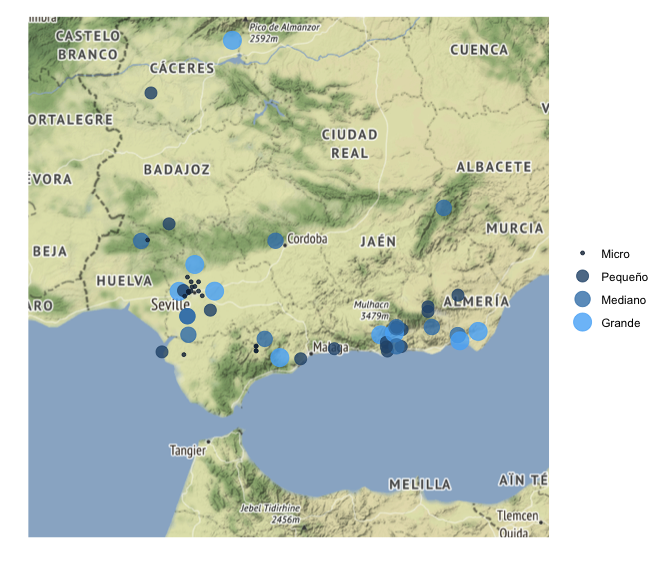
\includegraphics[width=0.9\linewidth]{figures/mapa-tomate} 

}

\caption[Mapa de entrevistados]{Distribución de los productores de tomate según tamaño de la SAU}\label{fig:mapa-tomate}
\end{figure}

\begin{table}

\caption[Caracterización de los entrevistados]{\label{tab:tabla-caracterizacion}Caracterización de agricultores entrevistados según factores sociodemográficos y técnico productivos.}
\centering
\begin{tabular}[t]{llrr}
\toprule
\textbf{Varbiale} & \textbf{Categoría} & \textbf{n} & \textbf{\%}\\
\midrule
\addlinespace[0.3em]
\multicolumn{4}{l}{\textbf{Sociodemográficos}}\\
\hline
\hspace{1em}Sexo & F & 18 & 33\\
\hspace{1em} & M & 37 & 67\\
\midrule
\hspace{1em}Edad & Joven & 24 & 44\\
\hspace{1em} & Experimentado & 31 & 56\\
\midrule
\hspace{1em}Origen & Neorrural & 29 & 53\\
\hspace{1em} & Rural & 26 & 47\\
\midrule
\hspace{1em}Estudios & Primario & 17 & 31\\
\hspace{1em} & Secundario & 15 & 27\\
\hspace{1em} & Universitario & 23 & 42\\
\midrule
\addlinespace[0.3em]
\multicolumn{4}{l}{\textbf{Técnicos productivos}}\\
\hline
\hspace{1em}Area & Micro & 24 & 44\\
\hspace{1em} & Pequeño & 18 & 33\\
\hspace{1em} & Mediano & 7 & 13\\
\hspace{1em} & Grande & 6 & 11\\
\midrule
\hspace{1em}Propia & No & 24 & 44\\
\hspace{1em} & Si & 31 & 56\\
\midrule
\hspace{1em}Variedades & 1 & 32 & 58\\
\hspace{1em} & 2 & 7 & 13\\
\hspace{1em} & 2+ & 16 & 29\\
\midrule
\hspace{1em}Invernadero & No & 38 & 69\\
\hspace{1em} & Si & 17 & 31\\
\bottomrule
\multicolumn{4}{l}{\textsuperscript{a} $n=55$}\\
\end{tabular}
\end{table}

\hypertarget{resultados}{%
\chapter{Resultados}\label{resultados}}

\minitoc 

\hypertarget{comparaciuxf3n-de-valoraciuxf3n-entre-las-pps}{%
\section{Comparación de valoración entre las PPs}\label{comparaciuxf3n-de-valoraciuxf3n-entre-las-pps}}

En la Figura \ref{fig:fig-todas-politicas} se muestran los porcentajes de respuesta por política, agrupadas por tipo de respuesta. En general, la PP que se mostró como más desconocida fue la Directiva de Nitratos y la que recibió mayor valoración como \emph{Útil} fue la Estrategia sobre la Biodiversidad 2030. Además se aprecia que la respuesta \emph{Inutil} es la que cuenta con menos frecuencia para todas las políticas.

\begin{figure}
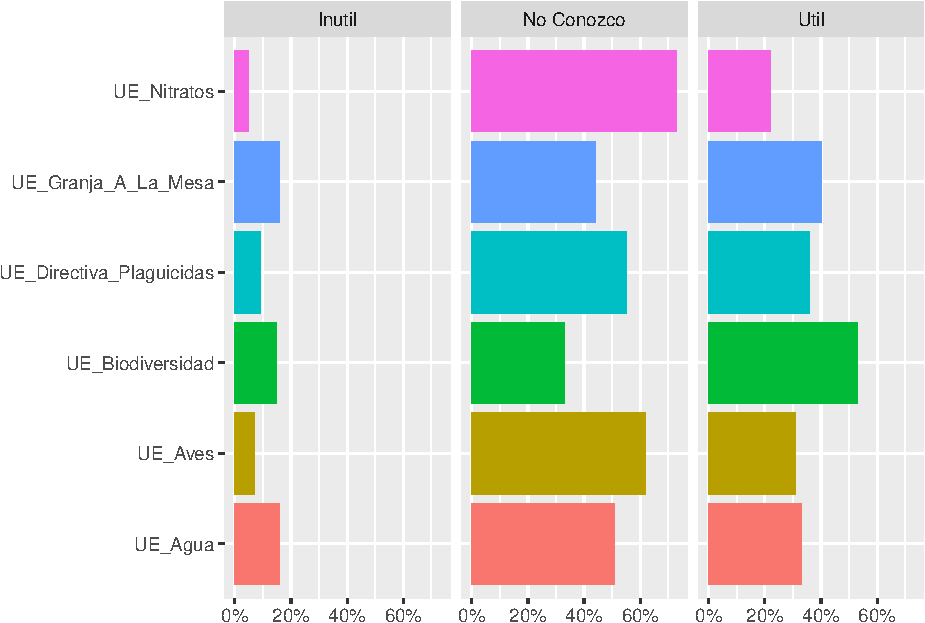
\includegraphics{_main_files/figure-latex/fig-todas-politicas-1} \caption[Políticas Públicas arupadas por respuesta]{Porcentaje de respuestas entre políticas, agrupadas por tipo de respuesta ($n=55$).}\label{fig:fig-todas-politicas}
\end{figure}

Al analizar las diferencias de valoración entre PPs agrupadas por parejas (Tabla \ref{tab:mcnemar-politicas} se encontraron 3 parejas con diferencias significativas de valoración. Además 6 comparaciones no pudieron analizarse debido al tamaño de la muestra (presencia de ceros en categorías) y pasaron directamente al análisis \emph{Posthoc}. De las 6 parejas, 2 tuvieron diferencias significativas (marcadas con un \(\bullet\)) dando un total de 5 parejas para el análisis \emph{Posthoc}. Las 4 parejas sin diferencias significativas fueron marcadads con \(0_s\).

\begin{table}

\caption[Comparación de percepeción entre PPs]{\label{tab:mcnemar-politicas}Valores p de las pruebas de simetría de McNemar-Bowker comparando parejas de PPs}
\centering
\begin{tabular}[t]{lllllll}
\toprule
  & Agua & Aves & Nitratos & Granja & Biodiversidad & Plaguicidas\\
\midrule
Agua & - & - & - & - & - & -\\
Aves & $\geq 0,05$ & - & - & - & - & -\\
Nitratos & \textbf{<0,01}$^{**}$ & $0_s$ & - & - & - & -\\
Granja & $\geq 0,05$ & $0_s$ & $\bullet$ & - & - & -\\
Biodiversidad & \textbf{<0,05}$^{*}$ & \textbf{<0,001}$^{***}$ & $\bullet$ & $\geq 0,05$ & - & -\\
\addlinespace
Plaguicidas & $\geq 0,05$ & $\geq 0,05$ & $0_s$ & $\geq 0,05$ & $0_s$ & -\\
\bottomrule
\multicolumn{7}{l}{\textsuperscript{a} Nivel de significancia ($p<0.05$) $\rightarrow$ Alto = ***, Medio = ** y Bajo = *}\\
\multicolumn{7}{l}{\textsuperscript{b} $\bullet \rightarrow$ limitación por presencia de y valores significativos en análisis $posthoc$}\\
\multicolumn{7}{l}{\textsuperscript{c} $0_s \rightarrow$ limitación por presencia de ceros y valores no significativos en análisis $posthoc$}\\
\end{tabular}
\end{table}

En el análisis \emph{Posthoc}, al comparar la simetría 2x2 de las respuestas de los 7 casos, 6 tuvieron diferencias significativas en el par \emph{No Conozco/No Conozco : Util/Util}.

En la Tabla \ref{tab:post-mcnemar} se muestran las tablas de contingencia para los 7 casos y se reportan los valores-p de las pruebas de McNemar y los valores-p del test de simetría 2x2 significativos. Los valores-p de los pares \emph{Inutil/Inutil : No Conozco/No Conozco} y \emph{Inutil/Inutil : Util/Util} no fueron reportados por no ser significativos. El caso de \emph{Nitratos vs Agua} es el único cuyo valor-p del par \emph{No Conozco/No Conozco : Util/Util} no es significativo pero se reporta por ser de información útil para el análisis \emph{Posthoc}.

\begin{table}[hbtp]
  \begin{threeparttable}
  \caption[Análisis Posthoc de las asociaciones entre PPs]{Tablas de contingencia de cada par de PP que explica la difrencia de percepción entre PPs según el test de McNemar} 
  \label{tab:post-mcnemar}
    \begin{tabular}{@{}c@{}} % dummy "outer" tabular env.
      \begin{minipage}{\textwidth}
        \begin{subtable}[b]{0.4\textwidth}

\begin{tabular}{llll}
\toprule
\multicolumn{1}{c}{\textbf{ }} & \multicolumn{3}{c}{\textbf{Nitratos}} \\
  & Inutil & No Conozco & Util\\
\midrule
\addlinespace[0.3em]
\multicolumn{4}{l}{\textbf{Agua}}\\
\hspace{1em}Inutil & 3 & 4 & 2\\
\hspace{1em}No Conozco & 0 & \textcolor{red}{27} & \textcolor{red}{1}\\
\hspace{1em}Util & 0 & \textcolor{red}{9} & \textcolor{red}{9}\\
\bottomrule
\multicolumn{4}{l}{\textsuperscript{a} p-valor McNemar: 0.006}\\
\multicolumn{4}{l}{\textsuperscript{b} p-valor Simetría 2x2: 0.081}\\
\end{tabular}
        \caption{}
        \label{tab:agua-nitratos}
        \end{subtable}
\hfill
        \begin{subtable}[b]{0.4\textwidth}

\begin{tabular}{llll}
\toprule
\multicolumn{1}{c}{\textbf{ }} & \multicolumn{3}{c}{\textbf{Biodiversidad}} \\
  & Inutil & No Conozco & Util\\
\midrule
\addlinespace[0.3em]
\multicolumn{4}{l}{\textbf{Agua}}\\
\hspace{1em}Inutil & 4 & 1 & 4\\
\hspace{1em}No Conozco & 2 & \textcolor{red}{16} & \textcolor{red}{10}\\
\hspace{1em}Util & 2 & \textcolor{red}{1} & \textcolor{red}{15}\\
\bottomrule
\multicolumn{4}{l}{\textsuperscript{a} p-valor McNemar: 0.039}\\
\multicolumn{4}{l}{\textsuperscript{b} p-valor Simetría 2x2: 0.048}\\
\end{tabular}
        \caption{}
        \label{tab:agua-biodiversidad}
        \end{subtable}
\hfill
        \begin{subtable}[b]{0.4\textwidth}

\begin{tabular}{llll}
\toprule
\multicolumn{1}{c}{\textbf{ }} & \multicolumn{3}{c}{\textbf{Granja}} \\
  & Inutil & No Conozco & Util\\
\midrule
\addlinespace[0.3em]
\multicolumn{4}{l}{\textbf{Nitratos}}\\
\hspace{1em}Inutil & 3 & 0 & 0\\
\hspace{1em}No Conozco & 6 & \textcolor{red}{23} & \textcolor{red}{11}\\
\hspace{1em}Util & 0 & \textcolor{red}{1} & \textcolor{red}{11}\\
\bottomrule
\multicolumn{4}{l}{\textsuperscript{a} p-valor McNemar: NaN}\\
\multicolumn{4}{l}{\textsuperscript{b} p-valor Simetría 2x2: 0.019}\\
\end{tabular}
        \caption{}
        \label{tab:nitratos-granja}
        \end{subtable}
\hfill
        \begin{subtable}[b]{0.4\textwidth}

\begin{tabular}{llll}
\toprule
\multicolumn{1}{c}{\textbf{ }} & \multicolumn{3}{c}{\textbf{Biodiversidad}} \\
  & Inutil & No Conozco & Util\\
\midrule
\addlinespace[0.3em]
\multicolumn{4}{l}{\textbf{Nitratos}}\\
\hspace{1em}Inutil & 3 & 0 & 0\\
\hspace{1em}No Conozco & 5 & \textcolor{red}{17} & \textcolor{red}{18}\\
\hspace{1em}Util & 0 & \textcolor{red}{1} & \textcolor{red}{11}\\
\bottomrule
\multicolumn{4}{l}{\textsuperscript{a} p-valor McNemar: NaN}\\
\multicolumn{4}{l}{\textsuperscript{b} p-valor Simetría 2x2: 5e-04}\\
\end{tabular}
        \caption{}
        \label{tab:nitratos-biodiversidad}
        \end{subtable}
\hfill
        \begin{subtable}[c]{\textwidth}
\centering

\begin{tabular}{llll}
\toprule
\multicolumn{1}{c}{\textbf{ }} & \multicolumn{3}{c}{\textbf{Biodiversidad}} \\
  & Inutil & No Conozco & Util\\
\midrule
\addlinespace[0.3em]
\multicolumn{4}{l}{\textbf{Aves}}\\
\hspace{1em}Inutil & 3 & 1 & 0\\
\hspace{1em}No Conozco & 3 & \textcolor{red}{17} & \textcolor{red}{14}\\
\hspace{1em}Util & 2 & \textcolor{red}{0} & \textcolor{red}{15}\\
\bottomrule
\multicolumn{4}{l}{\textsuperscript{a} p-valor McNemar: 0.001}\\
\multicolumn{4}{l}{\textsuperscript{b} p-valor Simetría 2x2: 0.002}\\
\end{tabular}
        \caption{}
        \label{tab:aves-biodiversidad}
        \end{subtable}
\bigskip
        \begin{tablenotes}
        \item[] \tikz\draw[red,fill=red] (0,0) circle (.5ex); Tablas 2x2 con valores p del test de simetría significativos.
        \end{tablenotes}
      \end{minipage}
    \end{tabular} % end of dummy "outer" tabular env.
\end{threeparttable}
\end{table}

\hypertarget{sociodemo-pps}{%
\section{Influencia de factores sociodemográficos en la valoración de las PPs}\label{sociodemo-pps}}

En el análisis de la asosiación entre factores sociodemográficos y las valoraciones de las PPs se encontraron 3 casos significativos para los factores ``Estudios'' y ``Origen'' (Tabla \ref{tab:socio-demograficos-politicas}).

\begin{table}[H]

\caption[Asociación entre factores sociodemográficos y PPs]{\label{tab:socio-demograficos-politicas}Valores p de las pruebas de Fisher para cada factor sociodemográfico y política }
\centering
\begin{tabular}[t]{lllllll}
\toprule
  & Agua & Aves & Nitratos & Granja & Biodiversidad & Plaguicidas\\
\midrule
Estudios & $\geq 0,05$ & $\geq 0,05$ & $\geq 0,05$ & \textbf{<0,05}$^{*}$ & $\geq 0,05$ & $\geq 0,05$\\
Joven & $\geq 0,05$ & $\geq 0,05$ & $\geq 0,05$ & $\geq 0,05$ & $\geq 0,05$ & $\geq 0,05$\\
Origen & $\geq 0,05$ & \textbf{<0,05}$^{*}$ & $\geq 0,05$ & \textbf{<0,05}$^{*}$ & $\geq 0,05$ & $\geq 0,05$\\
Sexo & $\geq 0,05$ & $\geq 0,05$ & $\geq 0,05$ & $\geq 0,05$ & $\geq 0,05$ & $\geq 0,05$\\
\bottomrule
\multicolumn{7}{l}{\textsuperscript{a} Nivel de significancia ($p<0.05$) $\rightarrow$ Alto = ***, Medio = ** y Bajo = *}\\
\end{tabular}
\end{table}

Para cada par factor sociodemográfico-política que resultó significativamente relacionado se reportaron las tablas de contingencia. Con el fin de analizar la tendencias de respuesta de los grupos dentro de cada factor se reportan en azul aquellas respuestas cuyos residuos estandarizados de la prueba de \({\chi}^2\) es significativa (Tablas \ref{tab:estudios-posthoc} y \ref{tab:origen-posthoc}). Además se reportaron asosiaciones positivas y negativas mediante un ``\(+\)'' y un ``\(-\)'' respectivamente. Por ejemplo en la Tabla \ref{tab:estudios-posthoc} se observa una asociación positiva entre la respuesta ``No Conozco'' y la categoría de estudio ``Secundario''.

\begin{table}[h!]
\caption[Asociación entre Estudios y PPs]{Tablas de contingencia donde el factor Estudios tuvo una asociación significativa con la PP "\textit{Granja}".}
\label{tab:estudios-posthoc}
 \centering
  \begin{threeparttable}

\begin{tabular}{llll}
\toprule
\multicolumn{1}{c}{\textbf{ }} & \multicolumn{3}{c}{\textbf{Estudios}} \\
  & Primario & Secundario & Universitario\\
\midrule
\addlinespace[0.3em]
\multicolumn{4}{l}{\textbf{Granja}}\\
\hspace{1em}Inutil & 5 & 2 & 2\\
\hspace{1em}No Conozco & 7 & \textcolor{blue}{\textbf{10 +$^{*}$}} & 7\\
\hspace{1em}Util & 5 & 3 & \textcolor{blue}{\textbf{10 +$^{**}$}}\\
\bottomrule
\end{tabular}
  \end{threeparttable}
  \quad
  \begin{minipage}{\linewidth}
     \begin{threeparttable}
      \begin{tablenotes}
      \item[a] \tikz\draw[blue,fill=blue] (0,0) circle (.5ex); Valores significativos, donde nivel de significancia ($p<0.05$) $\rightarrow$ Alto = ***, \newline 
      Medio = ** y Bajo = *
      \item[b] $+$ $\rightarrow$ Correlación positiva.
      \item[c] $-$ $\rightarrow$ Correlación negativa.
      \end{tablenotes}
     \end{threeparttable}
  \end{minipage}
\end{table}

\begin{table}
 \centering
  \begin{threeparttable}
  \caption[ASociación entre el factor Origen y PPs]{Tablas de contingencia donde el factor Origen tuvo una asosiación significativa con las PPs (a) "\textit{Aves}" y (b) "\textit{Granja}".}
\label{tab:origen-posthoc}
  \begin{tabular}{@{}c@{}} % dummy "outer" tabular env.
\begin{minipage}{\textwidth}

\begin{subtable}[b]{0.4\textwidth}


\begin{tabular}{lll}
\toprule
\multicolumn{1}{c}{\textbf{ }} & \multicolumn{2}{c}{\textbf{Origen}} \\
  & Neorrural & Rural\\
\midrule
\addlinespace[0.3em]
\multicolumn{3}{l}{\textbf{Aves}}\\
\hspace{1em}Inutil & \textcolor{blue}{\textbf{0 -$^{*}$}} & \textcolor{blue}{\textbf{4 +$^{*}$}}\\
\hspace{1em}No Conozco & 17 & 17\\
\hspace{1em}Util & 12 & 5\\
\bottomrule
\end{tabular}
  \caption{}
  \label{tab:origen-aves}
\end{subtable}
\hfill
 \begin{subtable}[b]{0.4\textwidth}

\begin{tabular}{lll}
\toprule
\multicolumn{1}{c}{\textbf{ }} & \multicolumn{2}{c}{\textbf{Origen}} \\
  & Neorrural & Rural\\
\midrule
\addlinespace[0.3em]
\multicolumn{3}{l}{\textbf{Granja}}\\
\hspace{1em}Inutil & \textcolor{blue}{\textbf{1 -$^{**}$}} & \textcolor{blue}{\textbf{8 +$^{**}$}}\\
\hspace{1em}No Conozco & 15 & 9\\
\hspace{1em}Util & 13 & 9\\
\bottomrule
\end{tabular}
    \caption{}
      \label{tab:origen-granja}
\end{subtable}
\hfill
\end{minipage}
\end{tabular} % end of dummy "outer" tabular env.
\end{threeparttable}

  \begin{minipage}{\linewidth}
     \begin{threeparttable}
      \begin{tablenotes}
      \item[a] \tikz\draw[blue,fill=blue] (0,0) circle (.5ex); Valores significativas, donde nivel de significancia ($p<0.05$) $\rightarrow$ Alto = ***, \newline 
      Medio = ** y Bajo = *
      \item[b] $+$ $\rightarrow$ Correlación positiva.
      \item[c] $-$ $\rightarrow$ Correlación negativa.
      \end{tablenotes}
     \end{threeparttable}
  \end{minipage}
\end{table}

\hypertarget{influencia-de-factores-tuxe9cnico-productivos-en-la-valoraciuxf3n-de-las-pps}{%
\section{Influencia de factores técnico productivos en la valoración de las PPs}\label{influencia-de-factores-tuxe9cnico-productivos-en-la-valoraciuxf3n-de-las-pps}}

Al igual que en la sección \ref{sociodemo-pps} se reportaron todos los valores-p para cada par factor-PP y se encontraron 5 casos significativos para los factores ``Área'' e ``Invernadero'' (Tabla \ref{tab:tecnico-productivos-politicas}).

\begin{table}[H]

\caption[Asociación entre factores técnicos productivos y PPs]{\label{tab:tecnico-productivos-politicas}Valores p de las pruebas de Fisher para cada factor técnico productivo y política }
\centering
\begin{tabular}[t]{lllllll}
\toprule
  & Agua & Aves & Nitratos & Granja & Biodiversidad & Plaguicidas\\
\midrule
Area & $\geq 0,05$ & $\geq 0,05$ & $\geq 0,05$ & \textbf{<0,01}$^{**}$ & $\geq 0,05$ & \textbf{<0,01}$^{**}$\\
Invernadero & \textbf{<0,05}$^{*}$ & \textbf{<0,05}$^{*}$ & \textbf{<0,05}$^{*}$ & $\geq 0,05$ & $\geq 0,05$ & $\geq 0,05$\\
Propia & $\geq 0,05$ & $\geq 0,05$ & $\geq 0,05$ & $\geq 0,05$ & $\geq 0,05$ & $\geq 0,05$\\
Variedades & $\geq 0,05$ & $\geq 0,05$ & $\geq 0,05$ & $\geq 0,05$ & $\geq 0,05$ & $\geq 0,05$\\
\bottomrule
\multicolumn{7}{l}{\textsuperscript{a} Nivel de significancia ($p<0.05$) $\rightarrow$ Alto = ***, Medio = ** y Bajo = *}\\
\end{tabular}
\end{table}

\begin{table}

 \centering
  \begin{threeparttable}
  \caption[Asociación entre el factor Área y PPs]{Tablas de contingencia donde el factor Area tuvo una asosiación significativa con alguna PP.}
  \label{tab:area-posthoc}
\begin{tabular}{@{}c@{}} % dummy "outer" tabular env.
\begin{minipage}{\textwidth}

\begin{subtable}[b]{\textwidth}
\centering

\begin{tabular}{lllll}
\toprule
\multicolumn{1}{c}{\textbf{ }} & \multicolumn{4}{c}{\textbf{Area}} \\
  & Micro & Pequeño & Mediano & Grande\\
\midrule
\addlinespace[0.3em]
\multicolumn{5}{l}{\textbf{Granja}}\\
\hspace{1em}Inutil & \textcolor{blue}{\textbf{0 -$^{**}$}} & 4 & 2 & \textcolor{blue}{\textbf{3 +$^{*}$}}\\
\hspace{1em}No Conozco & \textcolor{blue}{\textbf{17 +$^{***}$}} & 5 & 1 & 1\\
\hspace{1em}Util & 7 & 9 & 4 & 2\\
\bottomrule
\end{tabular}
 \caption{}
 \label{tab:area-granja}
\end{subtable}
\hfill

\begin{subtable}[b]{\textwidth}
\centering

\begin{tabular}{lllll}
\toprule
\multicolumn{1}{c}{\textbf{ }} & \multicolumn{4}{c}{\textbf{Area}} \\
  & Micro & Pequeño & Mediano & Grande\\
\midrule
\addlinespace[0.3em]
\multicolumn{5}{l}{\textbf{Plaguicidas}}\\
\hspace{1em}Inutil & 1 & 2 & 2 & 0\\
\hspace{1em}No Conozco & \textcolor{blue}{\textbf{18 +$^{**}$}} & 10 & \textcolor{blue}{\textbf{1 -$^{*}$}} & \textcolor{blue}{\textbf{1 -$^{*}$}}\\
\hspace{1em}Util & \textcolor{blue}{\textbf{5 -$^{*}$}} & 6 & 4 & \textcolor{blue}{\textbf{5 +$^{*}$}}\\
\bottomrule
\end{tabular}
 \caption{}
  \label{tab:area-plaguicidas}
\end{subtable}
\hfill
\end{minipage}
\end{tabular}
  \end{threeparttable}
  \begin{minipage}{\linewidth}
     \begin{threeparttable}
      \begin{tablenotes}
      \item[a] \tikz\draw[blue,fill=blue] (0,0) circle (.5ex); Valores significativas, donde nivel de significancia ($p<0.05$) $\rightarrow$ Alto = ***, \newline 
      Medio = ** y Bajo = *
      \item[b] $+$ $\rightarrow$ Correlación positiva.
      \item[c] $-$ $\rightarrow$ Correlación negativa.
      \end{tablenotes}
     \end{threeparttable}
  \end{minipage}
\end{table}

Para cada caso significativo se presentaron las tablas de contingencia resaltando en azul las respuestas con significancia para el análisis (Tabla \ref{tab:area-posthoc} y \ref{tab:invernadero-posthoc}).

\begin{table}
 \centering
  \begin{threeparttable}
  \caption[Asociación entre el factor Invernadero y PPs]{Tablas de contingencia donde el factor Invernadero tuvo una asosiación significativa con alguna PP.}
  \label{tab:invernadero-posthoc}
  \begin{tabular}{@{}c@{}} % dummy "outer" tabular env.
\begin{minipage}{\textwidth}

\begin{subtable}[b]{\textwidth}
\centering

\begin{tabular}{lll}
\toprule
\multicolumn{1}{c}{\textbf{ }} & \multicolumn{2}{c}{\textbf{Invernadero}} \\
  & FALSE & TRUE\\
\midrule
\addlinespace[0.3em]
\multicolumn{3}{l}{\textbf{Agua}}\\
\hspace{1em}Inutil & \textcolor{blue}{\textbf{3 -$^{*}$}} & \textcolor{blue}{\textbf{6 +$^{*}$}}\\
\hspace{1em}No Conozco & 22 & 6\\
\hspace{1em}Util & 13 & 5\\
\bottomrule
\end{tabular}
 \caption{}
 \label{tab:invernadero-agua}
\end{subtable}
\hfill
  
\begin{subtable}[b]{0.4\textwidth}

\begin{tabular}{lll}
\toprule
\multicolumn{1}{c}{\textbf{ }} & \multicolumn{2}{c}{\textbf{Invernadero}} \\
  & FALSE & TRUE\\
\midrule
\addlinespace[0.3em]
\multicolumn{3}{l}{\textbf{Aves}}\\
\hspace{1em}Inutil & \textcolor{blue}{\textbf{0 -$^{**}$}} & \textcolor{blue}{\textbf{4 +$^{**}$}}\\
\hspace{1em}No Conozco & 26 & 8\\
\hspace{1em}Util & 12 & 5\\
\bottomrule
\end{tabular}
  \caption{}
\label{tab:invernadero-aves}
\end{subtable}
\hfill
 \begin{subtable}[b]{0.4\textwidth}

\begin{tabular}{lll}
\toprule
\multicolumn{1}{c}{\textbf{ }} & \multicolumn{2}{c}{\textbf{Invernadero}} \\
  & FALSE & TRUE\\
\midrule
\addlinespace[0.3em]
\multicolumn{3}{l}{\textbf{Nitratos}}\\
\hspace{1em}Inutil & \textcolor{blue}{\textbf{0 -$^{**}$}} & \textcolor{blue}{\textbf{3 +$^{**}$}}\\
\hspace{1em}No Conozco & 30 & 10\\
\hspace{1em}Util & 8 & 4\\
\bottomrule
\end{tabular}
 \caption{}
 \label{tab:invernadero-nitratos}
\end{subtable}
\hfill
\end{minipage}
\end{tabular}
  \end{threeparttable}
  \begin{minipage}{\linewidth}
     \begin{threeparttable}
      \begin{tablenotes}
      \item[a] \tikz\draw[blue,fill=blue] (0,0) circle (.5ex); Valores significativas, donde nivel de significancia ($p<0.05$) $\rightarrow$ Alto = ***, \newline 
      Medio = ** y Bajo = *
      \item[b] $+$ $\rightarrow$ Correlación positiva.
      \item[c] $-$ $\rightarrow$ Correlación negativa.
      \end{tablenotes}
     \end{threeparttable}
  \end{minipage}
\end{table}

\hypertarget{discusion}{%
\chapter{Discusión}\label{discusion}}

\minitoc 

\hypertarget{disc-factores-distribucion}{%
\section{Elecciones de factores y distribución de la muestra}\label{disc-factores-distribucion}}

En la Tabla \ref{tab:tabla-caracterizacion} se puede ver que el 67\% de los encuestados fueron mujeres.
Esto por un lado, marca la brecha de género que existe en zonas rurales (Oedl-Wieser, 2015 ; Shortall, 2015) pero también un defecto a la hora de contactar nuevos agricultores a través del método ``bola de nieve''.
Debido a una falta de tiempo y recursos no fue posible la realización de una preselección de posibles encuestados que garantizara el balance de las categorías estudiadas.
Sorprendentemente el balance se consiguió para los factores asociados con la edad y el origen, estadística que no coincide con la realidad (Zagata \& Sutherland, 2015 ; Leonard et al., 2017).
Uno de los grandes problemas a la hora de plantear la transición hacia un nuevo régimen agroalimentario de base agroecológica es el recambio generacional.

En cuanto los factores técnicos productivos se puede observar una tendencia decreciente de casos a medida que aumenta el tamaño de la SAU.
Como se marcaba en la Sección \ref{agricultura-familiar} la base campesina constituye la mayoría de las explotaciones alrededor del mundo tanto en número como en cantidad de alimento producido.
Sin embargo, actualmente está en debate el papel que se le debe otorgar a los grandes productores a la hora de participar en la transición (Altieri \& Nicholls, 2020).
El bloqueo institucional que sufre el escalamiento de la agroecología podría ser inicialmente superado por grandes productores, generando luego un efecto de tracción con los productores más pequeños.

Los factores de \emph{``Sexo'', ``Edad'', ``Origen'' y ``Área''} fueron elegidos por considerarse actores fundamentales en la transformación del marco institucional a corto y mediano plazo (Recanati et al., 2019).
Los restantes, \emph{``Estudios,''Propia'', ``Variedades''e ``Invernadero''} fueron electos con un fin exploratorio.

\hypertarget{PPvsPP}{%
\section{Comparación entre Políticas Públicas}\label{PPvsPP}}

En la \ref{fig:fig-todas-politicas} se puede observar la primera tendencia general, el desconocimiento en general de las PPs.
Con la excepción de \emph{``Biodiversidad''}, la respuesta más popular fue \emph{``No conozco''}.
La segunda respuesta con mayor frecuencia fue \emph{``Útil''} y por último \emph{``Inútil''}.

A través de la Tabla \ref{tab:mcnemar-politicas} podemos observar que de las 15 posibilidades de combinación entre PPs, 5 tuvieron una diferencia significativa entre sus respuestas.
Esto quiere decir que la tendencia general de desconocimiento es válida.
En otras palabras, dos tercios de las posibilidades totales siguen un patrón ordenado descendentemente por desconocimiento, utilidad e inutilidad.

Al analizar el tercio restante de la Tabla \ref{tab:mcnemar-politicas}, se nota que los cambios de respuesta entre PPs oscila entre el desconocimiento y la utilidad.
En concreto, en la tabla \ref{tab:nitratos-biodiversidad}d de los 40 entrevistados que desconocieron la política de ``\emph{Nitratos''}, 18 (alrededor del 50\%) les pareció útil la de \emph{''Biodiversidad''}.
Estos resultados permiten dos posibles lecturas.
Por un lado, cuando los agricultores estan informados acerca de la PP, tienden a percibirla como útil antes que inútil.
Por otro lado, las nuevas PPs como \emph{''Biodiversidad''} tienen mayor difusión y su campaña de información es más eficiente frente a las PPs con mayor antigüedad.
Las tablas \ref{tab:agua-biodiversidad}b, \ref{tab:nitratos-biodiversidad}d y \ref{tab:aves-biodiversidad}e demuestran la efectividad de la campaña de difusión de \emph{''Biodiversidad''} frente a las PPs del siglo pasado:''\emph{Agua''}, ``\emph{Aves''} y''\emph{Nitratos''}.
La Tabla \ref{tab:nitratos-granja}c resiste un análisis similar, donde Granja es percibida de mayor utilidad que ``\emph{Nitratos''}.
En particular, el caso de la tabla Tabla \ref{tab:aves-biodiversidad}e demuestra la observación anterior ya que la PP de Biodiversidad puede entenderse como una actualización y ampliación de las PPs de \emph{``Aves''}.

Analizando en conjunto las Tablas \ref{tab:mcnemar-politicas}, \ref{tab:post-mcnemar} y la Figura \ref{fig:fig-todas-politicas} se puede observar que hay dos nodos de comparación entre las PPs.
En un extremo, \emph{``Biodiversidad''}, percibida como la de mayor utilidad y en el otro, \emph{``Nitratos''}, percibida como la más desconocida.

En definitiva, se observa que las campañas de información de las PPs son eficientes pero no suficientes.

\hypertarget{asociaciuxf3n-entre-factores-sociodemogruxe1ficos-y-poluxedticas-puxfablicas}{%
\section{Asociación entre factores sociodemográficos y Políticas Públicas}\label{asociaciuxf3n-entre-factores-sociodemogruxe1ficos-y-poluxedticas-puxfablicas}}

En la tabla 5.4 se observa que de los 24 casos estudiados, 3 resultaron asociados significativamente.
Dentro de esos 3, hubieron 2 factores en común: Estudios y Origen.

En el primer caso, el factor Estudios influye significativamente (Tabla \ref{tab:estudios-posthoc}) y hay una asociación positiva entre \emph{``Secundario: No Conozco''} y \emph{``Universitario: Util''}.
A pesar de que el análisis no es trasladable a las otras PPs, se puede observar el target de las nuevas campañas de difusión, donde a mayor nivel de estudio, mayor conocimiento y percepción de utilidad.

Ampliando la conclusión preliminar de la Sección \ref{PPvsPP}, la insuficiencia de las campañas de difusión de las PPs puede deberse a la imposibilidad de llegar a un público con menor formación.

El caso del factor \emph{``Origen''} permite una nueva lectura.
Tanto la Tabla \ref{tab:origen-aves}a como la \ref{tab:origen-granja}b asocian a un origen rural a la respuesta ``\emph{Inútil}'' de las PPs ``\emph{Granja}'' y ``\emph{Aves}'' respectivamente.
Mientras que los de origen neorrural tienen una asociación negativa a la respuesta ``\emph{Inútil}'' para ambos casos.
En base a este análisis se observa una pérdida de eficiencia en la comunicación de las PPs en los agricultores de origen rural.
Esto puede deberse a la resistencia al cambio de los agricultores con mayor experiencia pero también a que las PPs efectivamente no estan siendo eficientes en la resolución de los problemas del día a día, como por ejemplo el despoblamiento de zonas rurales o las grandes presiones económicas que llevan a la ruina a muchos de ellos.

\hypertarget{asociaciuxf3n-entre-factores-tuxe9cnicos-productivos-y-poluxedticas-puxfablicas}{%
\section{Asociación entre factores técnicos productivos y Políticas Públicas}\label{asociaciuxf3n-entre-factores-tuxe9cnicos-productivos-y-poluxedticas-puxfablicas}}

Al analizar la Tabla \ref{tab:tecnico-productivos-politicas} se observa que 5 de los 24 casos estudiados tuvieron asociaciones significativas.
De los 5, hubieron 2 factores en común: \emph{``Área''} e \emph{``Invernadero''}.

Analizando el factor \emph{``Área''}, la Tabla \ref{tab:area-posthoc} demuestra una de las grandes fallas en el diseño y la difusión de las PPs.
Tanto para el caso de ``\emph{Granja}'' y ``\emph{Plaguicidas}'', los micro productores se encuentran altamente asociados a la respuesta \emph{``No Conozco''}.
Paradójicamente una de las herramientas de la Estrategia de la Granja a la Mesa es la promoción de las cadenas cortas de distribución donde los micro productores juegan un papel fundamental.
Además como se marcó en la Sección \ref{agricultura-familiar} el campesinado y la agricultura familiar, generalmente asociada a micro y pequeñas producciones, debería ser el target principal en vistas de alcanzar los objetivos del \emph{PVE} y los \emph{ODS}.

Por otra parte, el factor \emph{``Invernadero''} se utilizó como un proxy de nivel de tecnificación.
La Tabla \ref{tab:invernadero-posthoc} muestra 3 resultados similares donde a mayor nivel de tecnificación se observa una tendencia hacia la percepción de inutilidad de las PPs \emph{``Agua''}, \emph{``Aves''} y \emph{``Nitratos''}.
Esto se podría deber a una mayor presión de los organismos de control sobre los agricultores más tecnificados.

\hypertarget{y-entonces-cuxf3mo-vamos}{%
\section{\texorpdfstring{\textquestiondown Y entonces? \textquestiondown Cómo vamos?}{Y entonces? Cómo vamos?}}\label{y-entonces-cuxf3mo-vamos}}

Durante el primer cuatrimestre del 2023 las emisiones de gases de efecto invernadero disminuyeron en un 2,9\% respecto al mismo cuatrimestre del 2022 (EUROSTAT, 2023).
Esta tendencia se condice con la disminución de emisiones desde finales del 2020, posiblemente por la implementación de las nuevas Políticas Públicas en el 2020 como la Estrategia de la Granja a la Mesa y la Estrategia sobre la Biodiversidad 2030.

Sin embargo hay evidencia científica que estos avances no son suficientes.
El mundo ya está 1,1 \(^{\circ}\)C más caliente que en la era preindustrial y los pronósticos del IPCC indican que el límite de 1,5\(^{\circ}\)C pactado en el PVE se alcanzará a inicios de la década del 2030 y para finales de siglo se alcanzará un aumento de entre 2 y 3 \(^{\circ}\)C frente a la era preindustrial (IPCC, 2023).

Por su parte, la UNEP ha publicado un seguimiento del avance de los ODS evidenciando la alarmante brecha entre el progreso actual y la meta fijada. Solamente los objetivos relacionados con el avance tecnológico, como por ejemplo el aumento del acceso a internet, demuestran avances considerables y en camino a llegar a buen puerto.
Particularmente los objetivos relacionados al sector agrícola, tales como Hambre Cero; Agua limpia y saneamiento; Acción el por el clima; Vida de ecosistemas terrestres, ponen evidencia un avance nulo o, aún más, un retroceso (UNEP, 2023).

Los datos oficiales y la percepción en general de los agricultores coinciden en que las nuevas PPs del sector agrícola tienen un impacto positivo pero no suficiente, ni para los objetivos globales, ni para el día a día de los agricultores.

\hypertarget{quuxe9-podemos-hacer}{%
\section{\texorpdfstring{\textquestiondown Qué podemos hacer?}{Qué podemos hacer?}}\label{quuxe9-podemos-hacer}}

La transición agroecológica se encuentra ante un bloqueo institucional que imposibilita su escalamiento.
Elinor Ostrom ha descripto 8 principios de diseño institucional asociados al manejo de los bienes comunes (Anderies \& Janssen, 2016) que nos ayudarán a diagnosticar el bloqueo y proponer posibles mejoras.
A continuación se describen 3 de ellos aplicados al tema de estudio:

\hypertarget{principio-n-circ-2-equivalencia-proporcional-entre-beneficios-y-costos.}{%
\subsection{\texorpdfstring{Principio N \(^{\circ}\) 2: Equivalencia proporcional entre beneficios y costos.}{Principio N \^{}\{\textbackslash circ\} 2: Equivalencia proporcional entre beneficios y costos.}}\label{principio-n-circ-2-equivalencia-proporcional-entre-beneficios-y-costos.}}

Uno de los principales problemas en el sector agrícola actual es la falta de recambio generacional y el abandono de tierras.
Este síntoma está íntimamente ligado al desbalance existente entre el esfuerzo productivo de los agricultores y el beneficio que obtienen a partir de ello.
Muchos jóvenes rurales deciden emigrar hacia centros urbanos en búsqueda de un futuro con mayor prosperidad económica (Kontogeorgos et al., 2015).
Al mismo tiempo, los productores de alimento, el primer eslabón de la cadena agroalimentaria, son los que reciben menores ingresos netos proporcionalmente debido a los altos costos de insumos y bajos precios de venta mayoristas.

Es necesario el reconocimiento y la puesta en valor de los agricultores en su conjunto mediante incentivos económicos que justifiquen el arduo y esencial trabajo en el campo.
La nueva \emph{Política Agraria Común} modificará los beneficios recibidos por cada actor del sector y serán necesarios mecanismos ágiles de diagnóstico que posibiliten la modificación de los incentivos en base a las necesidades locales (Principio N \(^{\circ}\) 6).

\hypertarget{principio-n-circ-3-acuerdos-de-elecciuxf3n-colectiva.}{%
\subsection{\texorpdfstring{Principio N \(^{\circ}\) 3: Acuerdos de elección colectiva.}{Principio N \^{}\{\textbackslash circ\} 3: Acuerdos de elección colectiva.}}\label{principio-n-circ-3-acuerdos-de-elecciuxf3n-colectiva.}}

Al diseñar PPs que deberán ser aplicadas a un gran territorio, como la UE, se dificulta la toma en cuenta de la diversidad de los allegados.
En menor medida se incorpora la opinión de los actores que habitan el territorio.
El alto desconocimiento de las PPs agrícolas por parte de los productores se basa en el incumplimiento de este principio.

Para aumentar el alcance efectivo de las PPs será necesario la co-creación de reglas, normas y estrategias entre el sector productivo y los organismos de control y decisión.
Afortunadamente el movimiento social agroecológico cuenta con la representatividad necesaria para proponer sesiones legislativas vinculantes en cada territorio.
Esencialmente nuevos mecanismos de gobernanza deberán idearse para el diseño de PPs que se adecuen a las necesidades territoriales.

\hypertarget{principio-n-circ-8-organismos-anidados.}{%
\subsection{\texorpdfstring{Principio N \(^{\circ}\) 8: Organismos anidados.}{Principio N \^{}\{\textbackslash circ\} 8: Organismos anidados.}}\label{principio-n-circ-8-organismos-anidados.}}

Este principio hace referencia a un sistema de gobernanza ``policéntrica''.
Se deberá evitar caer en la dicotomía entre la acción top-down (PPs) y bottom-up (acción social) creando instituciones con diferentes rangos de control: a nivel comunal, municipal, provincial, de comunidades autónomas y nacional.
Esta acción multinivel, en conjunto con el cumplimiento de los principios anteriores, posibilitarán un mecanismo de retroalimentación que podría otorgar resiliencia al nuevo marco normativo.

\hypertarget{posibles-mejoras-y-trabajo-futuro}{%
\section{Posibles mejoras y trabajo futuro}\label{posibles-mejoras-y-trabajo-futuro}}

Como se indicó en la Sección \ref{disc-factores-distribucion} para obtener resultados más fehacientes sería necesario primero ampliar el número de casos estudiados y luego realizar una selección de la muestra para que todas las categorías con valor de estudio estén balanceadas.

Por otro lado, gracias al trabajo de campo realizado se generó una base de datos con otras posibilidades de estudio que no pudieron ser exploradas por falta de tiempo. Además de las opiniones acerca de las PPs se consultó acerca de factores valorados con un indicador de tipo Likert que pueden ser agrupados en las siguientes 3 categorías:

\begin{itemize}
\tightlist
\item
  Consecuencias técnico productivas frente a la adopción del MIP.
\item
  Factores de importancia para la adopción de un control biológico de plagas.
\item
  Afirmaciones generales acerca de la percepción de la agricultura orgánica frente a la convencional.
\end{itemize}

Por último, sería necesaria la realización de un análisis estadístico multivariado combinando diferentes factores. Por ejemplo, si se estudiara \emph{``Sexo''} y \emph{``Origen''}: \textquestiondown Hay alguna diferencia de opinión entre las mujeres y los hombres neorrurales? \textquestiondown Y entre las mujeres neorrurales y los hombres rurales? Este tipo de análisis permitirá una mayor resolución para identificar posibles mejoras en base a una caracterización más exhaustiva.

Se deja a disposición el acceso al trabajo en \href{https://github.com/ipastore/TFM_AGE_UPO_IPB.git}{este repositorio de Github.} donde se puede encontrar la base de datos (\emph{.csv}), el cógido del análisis estadístico (\emph{R}) y la posibilidad de reproducir las figuras y tablas (\emph{RMarkdown}, \LaTeX).

\hypertarget{conclusion}{%
\chapter{Conclusión}\label{conclusion}}

Se han estudiado la opinión de 55 agricultores de tomate ecológico alrededor de Andalucía y Extremadura acerca de las PPs de la UE relacionadas al sector agrícola y se concluye que se confirman las 3 hipótesis planteadas. Por un lado, las PPs son percibidas con diferencias entre sí y por el otro, tanto los factores sociodemográficos como técnicos productivos están asociados a la percepción de los agricultores de las PPs.

Estas múltiples asociaciones pueden ayudar a esclarecer las razones por las cuales las PPs aplicadas hasta el día de la fecha resultan insuficientes para alcanzar los \emph{ODS} y las metas del \emph{PVE}. Al mismo tiempo que sirven como diagnóstico, conforman los cimientos para la modificación o desarrollo de futuras PPs que sean funcionales a las necesidades de los Pueblos y la Naturaleza.

\hypertarget{referencias}{%
\chapter*{Referencias}\label{referencias}}
\addcontentsline{toc}{chapter}{Referencias}

\markboth{Referencias}{}

\hypertarget{refs}{}
\begin{CSLReferences}{1}{0}
\leavevmode\vadjust pre{\hypertarget{ref-agnoletti2006}{}}%
Agnoletti, M. (2006). \emph{The conservation of cultural landscapes}. CABI Pub. \url{https://books.google.es/books?id=5QeSUdYvAjwC}

\leavevmode\vadjust pre{\hypertarget{ref-aguilera2020}{}}%
Aguilera, E., Díaz-Gaona, C., García-Laureano, R., Reyes-Palomo, C., Guzmán, G. I., Ortolani, L., Sánchez-Rodríguez, M., \& Rodríguez-Estévez, V. (2020). Agroecology for adaptation to climate change and resource depletion in the Mediterranean region. A review. \emph{Agricultural Systems}, \emph{181}, 102809. \url{https://doi.org/10.1016/j.agsy.2020.102809}

\leavevmode\vadjust pre{\hypertarget{ref-aguilera2019}{}}%
Aguilera, E., Vila-Traver, J., Deemer, B. R., Infante-Amate, J., Guzmán, G. I., \& González De Molina, M. (2019). Methane Emissions from Artificial Waterbodies Dominate the Carbon Footprint of Irrigation: A Study of Transitions in the Food{\textendash}Energy{\textendash}Water{\textendash}Climate Nexus (Spain, 1900{\textendash}2014). \emph{Environmental Science \& Technology}, \emph{53}(9), 5091--5101. \url{https://doi.org/10.1021/acs.est.9b00177}

\leavevmode\vadjust pre{\hypertarget{ref-altieri1987agroecology}{}}%
Altieri, M. A. (1987). \emph{Agroecology: The scientific basis of alternative agriculture} (p. 227). Westview Press, Boulder, CO.

\leavevmode\vadjust pre{\hypertarget{ref-altieri1989}{}}%
Altieri, M. A. (1989). \emph{Agroecology: A New Research and Development Paradigm for World Agriculture}.

\leavevmode\vadjust pre{\hypertarget{ref-altieri2020}{}}%
Altieri, M. A., \& Nicholls, C. I. (2020). Agroecology and the emergence of a post COVID-19 agriculture. \emph{Agriculture and Human Values}, \emph{37}(3), 525--526. \url{https://doi.org/10.1007/s10460-020-10043-7}

\leavevmode\vadjust pre{\hypertarget{ref-commons2021}{}}%
Anderies, J. M., \& Janssen, M. A. (2016). \emph{Sustaining the commons}. Center for Behavior, Institutions; the Environment. \url{https://sustainingthecommons.org/}

\leavevmode\vadjust pre{\hypertarget{ref-bensin1928agroecological}{}}%
Bensin, B. (1928). \emph{Agroecological characteristics description and classification of the local corn varieties}. Chorotypes.

\leavevmode\vadjust pre{\hypertarget{ref-campbell2017}{}}%
Campbell, B. M., Beare, D. J., Bennett, E. M., Hall-Spencer, J. M., Ingram, J. S. I., Jaramillo, F., Ortiz, R., Ramankutty, N., Sayer, J. A., \& Shindell, D. (2017). Agriculture production as a major driver of the Earth system exceeding planetary boundaries. \emph{Ecology and Society}, \emph{22}(4), art8. \url{https://doi.org/10.5751/ES-09595-220408}

\leavevmode\vadjust pre{\hypertarget{ref-carrascoandruxe9se.2014}{}}%
Carrasco, Andrés E. (2014). \emph{Declaración latinoamericana por una ciencia digna}. \url{https://www.biodiversidadla.org/Documentos/Declaracion_Latinoamericana_por_una_Ciencia_Digna_-_Por_la_prohibicion_de_los_transgenicos_en_Latinoamerica}

\leavevmode\vadjust pre{\hypertarget{ref-cordell2010}{}}%
Cordell, D. (2010). \emph{The story of phosphorus: sustainability implications of global phosphorus scarcity for food security}. Department of Water; Environmental Studies {[}The Tema Institute{]}, Linköping University.

\leavevmode\vadjust pre{\hypertarget{ref-crutzen2021}{}}%
Crutzen, P. J., \& Stoermer, E. F. (2021). \emph{The {``anthropocene''} (2000)} (S. Benner, G. Lax, P. J. Crutzen, U. Pöschl, J. Lelieveld, \& H. G. Brauch, Eds.; p. 1921). Springer International Publishing. \url{https://doi.org/10.1007/978-3-030-82202-6_2}

\leavevmode\vadjust pre{\hypertarget{ref-deschutter2011agroecology}{}}%
De Schutter, O. et al. (2011). Agroecology and the right to food. \emph{Report Presented at the 16th Session of the United Nations Human Rights Council {[}A/HRC/16/49{]}}, \emph{8}.

\leavevmode\vadjust pre{\hypertarget{ref-eurostat2023}{}}%
EUROSTAT. (2023). \emph{Air emissions accounts for greenhouse gases by NACE rev. 2 activity - quarterly data}. \url{https://ec.europa.eu/eurostat/databrowser/view/ENV_AC_AIGG_Q__custom_2691128/bookmark/table?lang=en&bookmarkId=4bb9ab20-296b-4119-88e9-580ea7741c0a}

\leavevmode\vadjust pre{\hypertarget{ref-thestat2023}{}}%
FAO. (2023). \emph{The State of Food Security and Nutrition in the World 2023}. FAO; IFAD; UNICEF; WFP; WHO; \url{https://doi.org/10.4060/cc3017en}

\leavevmode\vadjust pre{\hypertarget{ref-foley2005}{}}%
Foley, J. A., DeFries, R., Asner, G. P., Barford, C., Bonan, G., Carpenter, S. R., Chapin, F. S., Coe, M. T., Daily, G. C., Gibbs, H. K., Helkowski, J. H., Holloway, T., Howard, E. A., Kucharik, C. J., Monfreda, C., Patz, J. A., Prentice, I. C., Ramankutty, N., \& Snyder, P. K. (2005). Global Consequences of Land Use. \emph{Science}, \emph{309}(5734), 570--574. \url{https://doi.org/10.1126/science.1111772}

\leavevmode\vadjust pre{\hypertarget{ref-garridopeuxf1afrancisco2007}{}}%
Garrido Peña, F., González de Molina, M., Serrano, J. L., \& Solana, J. L. (eds. ). (2007). \emph{El paradigma ecológico en las ciencias sociales}. Icaria.

\leavevmode\vadjust pre{\hypertarget{ref-gliessman1990agroecology}{}}%
Gliessman, S. R. (1990). Agroecology: Researching the ecological basis for sustainable agriculture. In \emph{Agroecology: Researching the ecological basis for sustainable agriculture} (pp. 3--10). Springer.

\leavevmode\vadjust pre{\hypertarget{ref-demolina2021}{}}%
González de Molina, M., Petersen, P. F., Peña, F. G., \& Caporal, F. R. (2021). \emph{Introducción a la agroecología política}. Consejo Latinoamericano de Ciencias Sociales. CLACSO. \url{https://doi.org/10.2307/j.ctv2v88fc8}

\leavevmode\vadjust pre{\hypertarget{ref-gonzuxe1lezdemolina2014}{}}%
González de Molina, M., \& Toledo, V. M. (2014). \emph{The social metabolism: A socio-ecological theory of historical change} (1st ed. 2014). Springer International Publishing : Imprint: Springer. \url{https://doi.org/10.1007/978-3-319-06358-4}

\leavevmode\vadjust pre{\hypertarget{ref-guzmuxe1ncasado2009}{}}%
Guzmán Casado, G. I., \& González De Molina, M. (2009). Preindustrial agriculture versus organic agriculture. \emph{Land Use Policy}, \emph{26}(2), 502--510. \url{https://doi.org/10.1016/j.landusepol.2008.07.004}

\leavevmode\vadjust pre{\hypertarget{ref-guzman2000}{}}%
Guzmán Casado, G. I., Molina, M., \& Guzmán, E. (2000). \emph{Introducción a la agroecología como desarrollo rural sostenible} (p. 535). Ed: Mundi-Prensa. Madrid.

\leavevmode\vadjust pre{\hypertarget{ref-hall2011introduction}{}}%
Hall, C. A. (2011). Introduction to special issue on new studies in EROI (energy return on investment). In \emph{Sustainability} (No. 10; Vol. 3, pp. 1773--1777). Molecular Diversity Preservation International (MDPI).

\leavevmode\vadjust pre{\hypertarget{ref-hall2009minimum}{}}%
Hall, C. A., Balogh, S., \& Murphy, D. J. (2009). What is the minimum EROI that a sustainable society must have? \emph{Energies}, \emph{2}(1), 25--47.

\leavevmode\vadjust pre{\hypertarget{ref-hecht1995evolution}{}}%
Hecht, S. B. (1995). The evolution of agroecological thought. In \emph{Agroecology} (pp. 1--19). CRC Press.

\leavevmode\vadjust pre{\hypertarget{ref-henin1967acquisitions}{}}%
Hénin, S. (1967). Les acquisitions techniques en production v{é}g{é}tale et leur application. \emph{{É}conomie Rurale}, \emph{74}(1), 37--44.

\leavevmode\vadjust pre{\hypertarget{ref-HLPE12}{}}%
HLPE. (2017). \emph{Nutrition and food systems. A report by the high level panel of experts on food security and nutrition of the committee on world food security.} Rome.

\leavevmode\vadjust pre{\hypertarget{ref-holt2013agroecology}{}}%
Holt-Giménez, E., \& Altieri, M. A. (2013). Agroecology, food sovereignty, and the new green revolution. \emph{Agroecology and Sustainable Food Systems}, \emph{37}(1), 90--102.

\leavevmode\vadjust pre{\hypertarget{ref-king1956nuclear}{}}%
Hubbert M, K. (1956). Nuclear energy and the fossil fuels. \emph{American Petroleum Institute. Publication}, \emph{95}, 1--40.

\leavevmode\vadjust pre{\hypertarget{ref-iaastd2009}{}}%
International Assessment of Agricultural Knowledge Science and Technology for Development (IAASTD), U. N. E. P. (2009). \emph{Agriculture at a crossroads: Synthesis report}. \url{https://wedocs.unep.org/20.500.11822/7862}

\leavevmode\vadjust pre{\hypertarget{ref-change2019land}{}}%
IPCC. (2019). Land: An IPCC special report on climate change. In \emph{Desertification, land degradation, sustainable land management, food security, and greenhouse gas fluxes in terrestrial ecosystems} (Vol. 41).

\leavevmode\vadjust pre{\hypertarget{ref-IPCC2023}{}}%
IPCC. (2023). \emph{Climate change 2023: Synthesis report.} \url{https://doi.org/10.59327/IPCC/AR6-9789291691647}

\leavevmode\vadjust pre{\hypertarget{ref-kontogeorgos2015}{}}%
Kontogeorgos, A., Tsampra, M., \& Chatzitheodoridis, F. (2015). Agricultural policy and the environment protection through the eyes of new farmers: Evidence from a country of southeast europe. \emph{The Economies of Balkan and Eastern Europe Countries in the Changed World (EBEEC 2014)}, \emph{19}, 296--303. \url{https://doi.org/10.1016/S2212-5671(15)00030-1}

\leavevmode\vadjust pre{\hypertarget{ref-laherruxe8re2022}{}}%
Laherrère, J., Hall, C. A. S., \& Bentley, R. (2022). How much oil remains for the world to produce? Comparing assessment methods, and separating fact from fiction. \emph{Current Research in Environmental Sustainability}, \emph{4}, 100174. \url{https://doi.org/10.1016/j.crsust.2022.100174}

\leavevmode\vadjust pre{\hypertarget{ref-leonard2017}{}}%
Leonard, B., Kinsella, A., O'Donoghue, C., Farrell, M., \& Mahon, M. (2017). Policy drivers of farm succession and inheritance. \emph{Land Use Policy}, \emph{61}, 147--159. https://doi.org/\url{https://doi.org/10.1016/j.landusepol.2016.09.006}

\leavevmode\vadjust pre{\hypertarget{ref-levidow2014}{}}%
Levidow, L., Pimbert, M., \& Vanloqueren, G. (2014). Agroecological Research: Conforming{\textemdash}or Transforming the Dominant Agro-Food Regime? \emph{Agroecology and Sustainable Food Systems}, \emph{38}(10), 1127--1155. \url{https://doi.org/10.1080/21683565.2014.951459}

\leavevmode\vadjust pre{\hypertarget{ref-lowder2016}{}}%
Lowder, S. K., Skoet, J., \& Raney, T. (2016). The number, size, and distribution of farms, smallholder farms, and family farms worldwide. \emph{World Development}, \emph{87}, 16--29. https://doi.org/\url{https://doi.org/10.1016/j.worlddev.2015.10.041}

\leavevmode\vadjust pre{\hypertarget{ref-lyngsOxforddown2019}{}}%
Lyngs, U. (2019). Oxforddown: An oxford university thesis template for r markdown. In \emph{GitHub repository}. \url{https://github.com/ulyngs/oxforddown}; GitHub. \url{https://doi.org/10.5281/zenodo.3484682}

\leavevmode\vadjust pre{\hypertarget{ref-handbook-R-Man}{}}%
Mangiafico, S. (2016). \emph{Summary and analysis of extension program evaluation in r}.

\leavevmode\vadjust pre{\hypertarget{ref-mcmichael2006feeding}{}}%
McMichael, P. (2006). Feeding the world: Agriculture, development and ecology. In \emph{Socialist register 2007} (Vol. 43, pp. 170--194). Londres: Merlin Press.

\leavevmode\vadjust pre{\hypertarget{ref-muxe9ndez2013}{}}%
Méndez, V. E., Bacon, C. M., \& Cohen, R. (2013). Agroecology as a Transdisciplinary, Participatory, and Action-Oriented Approach. \emph{Agroecology and Sustainable Food Systems}, \emph{37}(1), 3--18. \url{https://doi.org/10.1080/10440046.2012.736926}

\leavevmode\vadjust pre{\hypertarget{ref-oedl2015}{}}%
Oedl-Wieser, T. (2015). Gender equality: A core dimension in rural development programmes in austria? \emph{Gender, Place \& Culture}, \emph{22}(5), 685--699. \url{https://doi.org/10.1080/0966369X.2013.879103}

\leavevmode\vadjust pre{\hypertarget{ref-ostrom1990governing}{}}%
Ostrom, E. (1990). \emph{Governing the commons: The evolution of institutions for collective action}. Cambridge university press.

\leavevmode\vadjust pre{\hypertarget{ref-ostrom2001commons}{}}%
Ostrom, E. (2001). \emph{Commons, institutional diversity of. Encyclopedia of biodiversity, volume i}. Academic Press.

\leavevmode\vadjust pre{\hypertarget{ref-ostrom2009}{}}%
Ostrom, E. (2009). A General Framework for Analyzing Sustainability of Social-Ecological Systems. \emph{Science}, \emph{325}(5939), 419--422. \url{https://doi.org/10.1126/science.1172133}

\leavevmode\vadjust pre{\hypertarget{ref-recanati2019}{}}%
Recanati, F., Maughan, C., Pedrotti, M., Dembska, K., \& Antonelli, M. (2019). Assessing the role of CAP for more sustainable and healthier food systems in Europe: A literature review. \emph{Science of The Total Environment}, \emph{653}, 908--919. \url{https://doi.org/10.1016/j.scitotenv.2018.10.377}

\leavevmode\vadjust pre{\hypertarget{ref-rockstrom2009planetary}{}}%
Rockstrom, J., Steffen, W., Noone, K., Persson, A., Chapin III, F. S., Lambin, E., Lenton, T. M., Scheffer, M., Folke, C., Schellnhuber, H. J., et al. (2009). Planetary boundaries: Exploring the safe operating space for humanity. \emph{Ecology and Society}, \emph{14}, 1--33.

\leavevmode\vadjust pre{\hypertarget{ref-schneidewind2016pledge}{}}%
Schneidewind, U., Singer-Brodowski, M., Augenstein, K., \& Stelzer, F. (2016). \emph{Pledge for a transformative science: A conceptual framework}.

\leavevmode\vadjust pre{\hypertarget{ref-shearman2012}{}}%
Shearman, P., Bryan, J., \& Laurance, W. F. (2012). Are we approaching {`}peak timber{'} in the tropics? \emph{Biological Conservation}, \emph{151}(1), 17--21. \url{https://doi.org/10.1016/j.biocon.2011.10.036}

\leavevmode\vadjust pre{\hypertarget{ref-shiva1989violence}{}}%
Shiva, V. (1989). The violence of the green revolution: Ecological degradation and political conflict in punjab. \emph{(No Title)}.

\leavevmode\vadjust pre{\hypertarget{ref-shortall2015}{}}%
Shortall, S. (2015). Gender mainstreaming and the common agricultural policy. \emph{Gender, Place \& Culture}, \emph{22}(5), 717--730. \url{https://doi.org/10.1080/0966369X.2014.939147}

\leavevmode\vadjust pre{\hypertarget{ref-steffen2015}{}}%
Steffen, W., Richardson, K., Rockström, J., Cornell, S. E., Fetzer, I., Bennett, E. M., Biggs, R., Carpenter, S. R., De Vries, W., De Wit, C. A., Folke, C., Gerten, D., Heinke, J., Mace, G. M., Persson, L. M., Ramanathan, V., Reyers, B., \& Sörlin, S. (2015). Planetary boundaries: Guiding human development on a changing planet. \emph{Science}, \emph{347}(6223), 1259855. \url{https://doi.org/10.1126/science.1259855}

\leavevmode\vadjust pre{\hypertarget{ref-tilman2001}{}}%
Tilman, D., Fargione, J., Wolff, B., D'Antonio, C., Dobson, A., Howarth, R., Schindler, D., Schlesinger, W. H., Simberloff, D., \& Swackhamer, D. (2001). Forecasting Agriculturally Driven Global Environmental Change. \emph{Science}, \emph{292}(5515), 281--284. \url{https://doi.org/10.1126/science.1057544}

\leavevmode\vadjust pre{\hypertarget{ref-toledo2012grandes}{}}%
Toledo, V. M. (2012). Los grandes problemas ecol{ó}gicos. \emph{Armando Bartra}, 29--34.

\leavevmode\vadjust pre{\hypertarget{ref-UNEP2023}{}}%
UNEP. (2023). \emph{Global sustainable development report 2023: Times of crisis, times of change: Science for accelerating transformations to sustainable development.}

\leavevmode\vadjust pre{\hypertarget{ref-united2011decoupling}{}}%
UNEP, I. (2011). \emph{Decoupling natural resource use and environmental impacts from economic growth}. UNEP/Earthprint.

\leavevmode\vadjust pre{\hypertarget{ref-unep2016global}{}}%
UNEP, I., Fischer-Kowalski, M., West, J., Giljum, S., Dittrich, M., \& Eisenmenger, N. (2016). Global material flows and resource productivity. \emph{Assessment Report for the UNEP International Resource Panel. United Nations Environment Programme, Nairobi}.

\leavevmode\vadjust pre{\hypertarget{ref-valerocapilla2015}{}}%
Valero Capilla, A., \& Valero Delgado, A. (2015). \emph{Thanatia: the destiny of the Earth's mineral resources: a cradle-to-cradle thermodynamic assessment}. World Scientific.

\leavevmode\vadjust pre{\hypertarget{ref-weis2013}{}}%
Weis, A. J. (2013). \emph{The ecological hoofprint: The global burden of industrial livestock}. Zed Books.

\leavevmode\vadjust pre{\hypertarget{ref-wezel2009}{}}%
Wezel, A., \& Soldat, V. (2009). A quantitative and qualitative historical analysis of the scientific discipline of agroecology. \emph{International Journal of Agricultural Sustainability}, \emph{7}(1), 3--18. \url{https://doi.org/10.3763/ijas.2009.0400}

\leavevmode\vadjust pre{\hypertarget{ref-worldbankgroup2022}{}}%
World Bank, G. (2022). Commodity markets outlook: The impact of the war in ukraine on commodity markets. \emph{World Bank, Washington, DC. License: Creative Commons Attribution CC BY 3.0 IGO.}

\leavevmode\vadjust pre{\hypertarget{ref-zagata2015}{}}%
Zagata, L., \& Sutherland, L.-A. (2015). Deconstructing the {`}young farmer problem in europe{'}: Towards a research agenda. \emph{Journal of Rural Studies}, \emph{38}, 39--51. https://doi.org/\url{https://doi.org/10.1016/j.jrurstud.2015.01.003}

\end{CSLReferences}

%%%%% REFERENCES

%%Para citar todo
\nocite{*}



\end{document}
